\documentclass{simcenterdocumentation}
\usepackage[backend=biber]{biblatex}
%\usepackage{subfig}
\usepackage{subcaption}
\usepackage{multirow}
\usepackage{adjustbox}
\usepackage{cleveref}
\usepackage{longtable}

%% SETTING ENVIRONMENT FOR PYTHON CODE SNIPPETS %%%%%%%%%%%%%%%%%%%%%%%%%%%%%%% 
\usepackage[utf8]{inputenc}

\graphicspath{{../Common/}{.}} %Setting the graphicspath
\makeatletter % Search additional directories for inputs
\def\input@path{{../Common/}{.}}
%or: \def\input@path{{/path/to/folder/}{/path/to/other/folder/}}
\makeatother

%%%%%%%%%%%%%%%%%%%%%%%%%%%%%%%%%%%%%%%%%%%%%%%%%%%%%%%%%%%%%%%%%%%%%%%%%%%%%%% 

% To compile this file, run "latex/pdflatex codedoc", then "biber codedoc"
% (or "bibtex codedoc", if the output from latex asks for that instead),
% and then "latex/pdflatex codedoc" (without the quotes in each case).

% Double spacing, if you want it.  Do not use for the final copy. Can also specify
% draft as a document class option. This will generate double spacing and placeholders
% for title page and header images
%% \def\dsp{\def\baselinestretch{2.0}\large\normalsize}
%% \dsp

\bibliography{../Common/references}

\begin{document}

% Declarations for Front Matter
% Software title followed by optional second line
\title{quoFEM\\ \Large Quantification of Uncertainty \& Optimization in Finite Element Modeling}
% Use superscripts to indicate author affiliations
\author{Frank McKenna, Nikhil Padhye, \& Adam Zsarnoczay}
%\author{Moe Howard$^{1,2}$ Larry Fine$^1$ Curly Howard$^2$}
\institutions{NHERI SimCenter, UC Berkeley}
\softwarename{quoFEM}
\softwareversion{1.2}
\softwarepage{https://simcenter.designsafe-ci.org/research-tools/uqfem-application/}

%%% DON'T MESS WITH THESE SETTINGS %%%%%%%%%%%%%%%%%%%%%%%%%%%%%%%%
\hypersetup{pageanchor=false}
\maketitle
\copyrightpage
\acknowledgments

\hypersetup{pageanchor=true}
\begin{frontmatter}

\pagestyle{plain}
{
  \renewcommand{\thispagestyle}[1]{}
  \tableofcontents
  \clearpage
  \listoffigures
  \clearpage
  \listoftables
}

\end{frontmatter}
\pagestyle{somewhatsimple}
%%%%%%%%%%%%%%%%%%%%%%%%%%%%%%%%%%%%%%%%%%%%%%%%%%%%%%%%%%%%%%%%%%%
% Create separate tex files for each chapter and provide them as inputs

\chapter{About}
\label{chap:about}
The quoFEM is an opensource software tool that allows engineers to incorporate uncertainty quantification to natural hazards. It has been developed at the SimCenter, within the University of California, Berkeley. The SimCenter is part of the Natural Hazards Engineering Research Infrastructure (NHERI) program, funded by the National Science Foundation. 

The intended audience for this tool is researchers and practitioners interested in predicting the response of a system under uncertainty. This documentation summarizes the usability and capabilities of this software tool.  Major enhancements are expected to be included in future releases of quoFEM.

This open-source research application, the source code of which is
available at
the \href{https://github.com/NHERI-SimCenter/EE-UQ}{\texttt{\getsoftwarename{}}
Github page}, provides an application that can be used to predict the
response of a system under uncertainty. The application
is focused on quantifying the uncertainties in the predicted response.
 In this application, the user is required to
characterize the uncertainties in the input. The application will,
after utilizing the users selected sampling method, provide
information that characterizes the uncertainties in the computed
response measures. As the computations to make these determinations
can be prohibitively expensive to perform on a user's local computer,
the user has the option to perform the computations remotely on the
Stampede2 supercomputer. Stampede2 is located at the Texas Advanced
Computing Center (TACC) and made available to the user through NHERI
DesignSafe, the cyberinfrastructure provider for the distributed NSF
funded Natural Hazards in Engineering Research Infrastructure (NHERI)
facility.\\

Whether running locally or remotely, the computations are performed, in a workflow
application. The design of the \texttt{\getsoftwarename{}} application is such that researchers are able to modify the backend application to utilize their own application in the workflow
computations. This will ensure researchers are not limited to using
the default applications we provide and will be enthused to provide
their own applications for others to use. \\

This document covers Version \getsoftwareversion{} of the tool. Users are
encouraged to comment on what additional features and capabilities
they would like to see in this application. These requests and
feedback can be submitted through an anonymous \insertsurveylink{user
survey}; we greatly appreciate any input you have. If there are
features you want, chances are many of your colleagues also would
benefit from them. Users are encouraged to review
\Cref{chap:requirements} to see what features are planned for this
application.


\chapter{Installation Instructions}
\label{chap:installation}
All SimCenter applications are available at
the \href{https://simcenter.designsafe-ci.org/research-tools/overview/}{SimCenter
website} under \emph{Research Tools}. The following sections outline
the steps necessary to download and install the \texttt{\getsoftwarename{}}
application. The SimCenter applications do require that you install a
number of other applications that are needed to run the workflows on
your local machine as well as at DesignSafe. \\


%===============================================================================
\section{Download the Application}
%===============================================================================

% \subsection{Download the Application Files}

To download the \texttt{\getsoftwarename{}} application navigate to
the \getsoftwarepage{\texttt{\getsoftwarename{}} page} and click on
the \emph{Download App \& User Manual} link on the right side of the
page. As shown in \Cref{fig:app_choose_file}, this will bring you to another page which contains a list of downloadable files and directories.

\softwareSwitch{PBE}{
\begin{figure}[!htbp]
  \centering {
    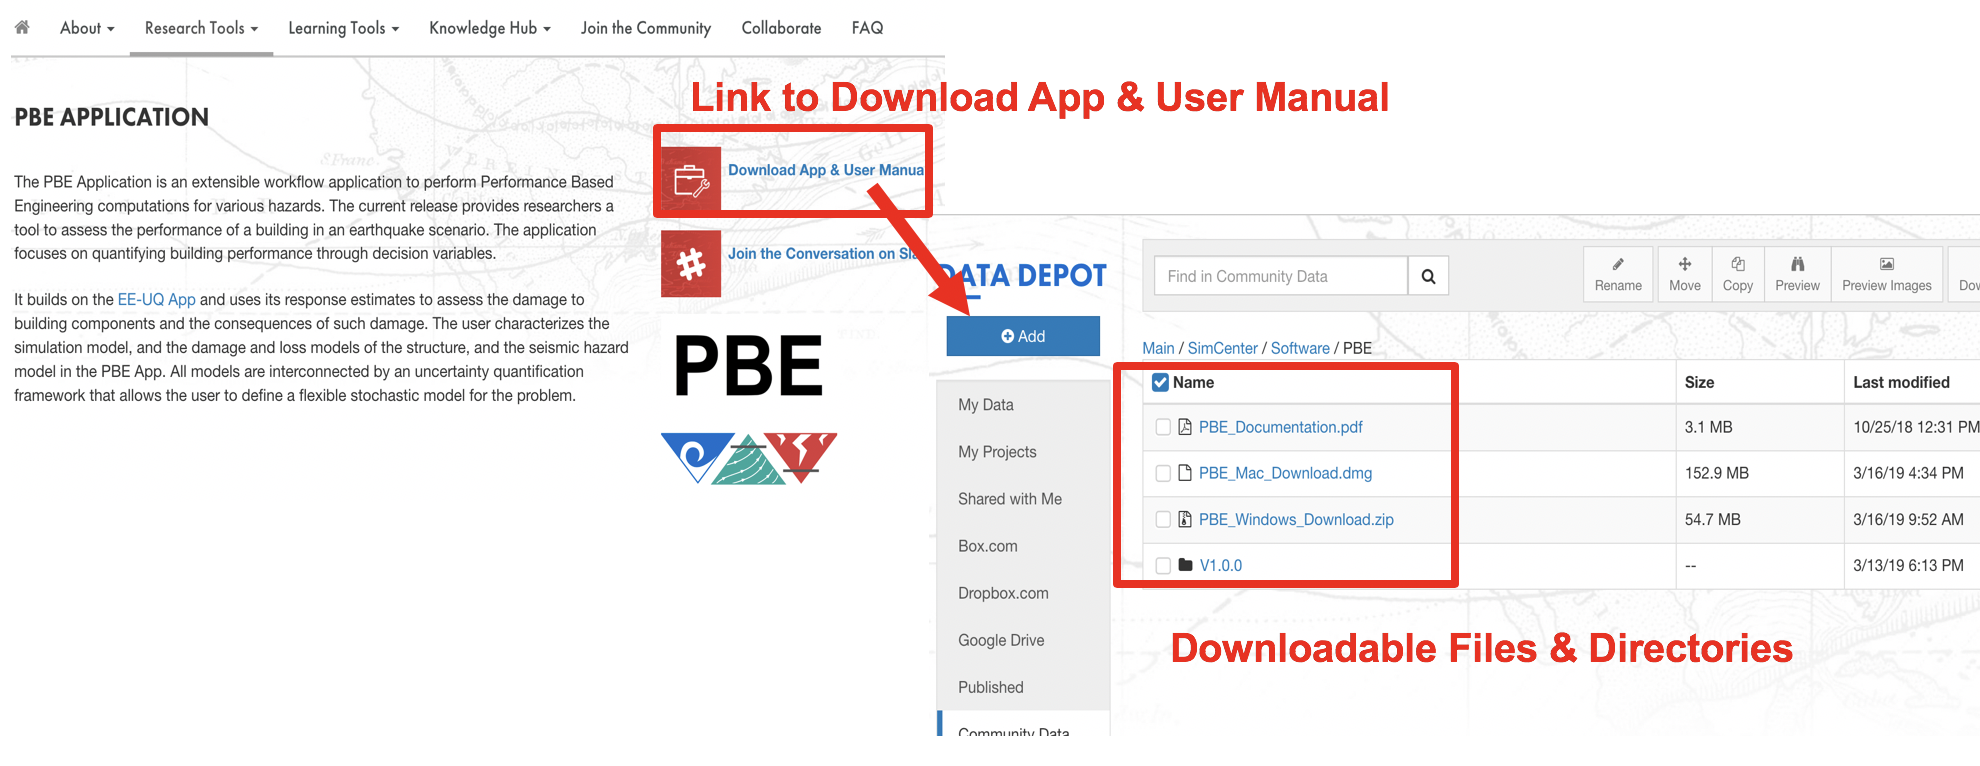
\includegraphics[width=0.95\textwidth]
    {installation/figures/pbeDownload.png} }
  \caption{Download Application}
  \label{fig:app_choose_file}
\end{figure}
}{}

\softwareSwitch{EE-UQ}{
\begin{figure}[!htbp]
  \centering {
    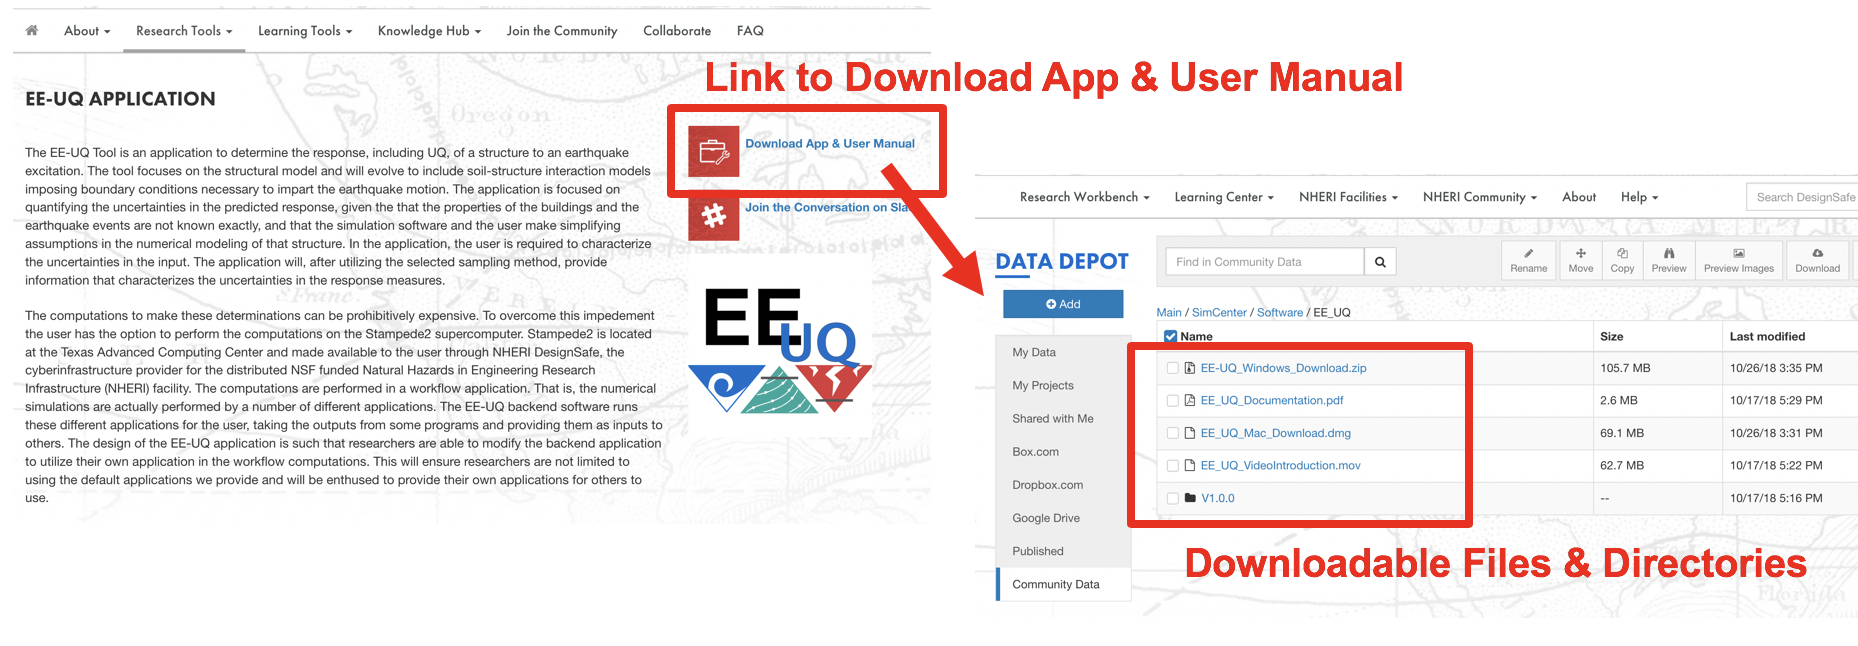
\includegraphics[width=0.95\textwidth]
    {installation/figures/eeDownload.png} }
  \caption{Download Application}
  \label{fig:app_choose_file}
\end{figure}
}{}

\softwareSwitch{WE-UQ}{
\begin{figure}[!htbp]
  \centering {
    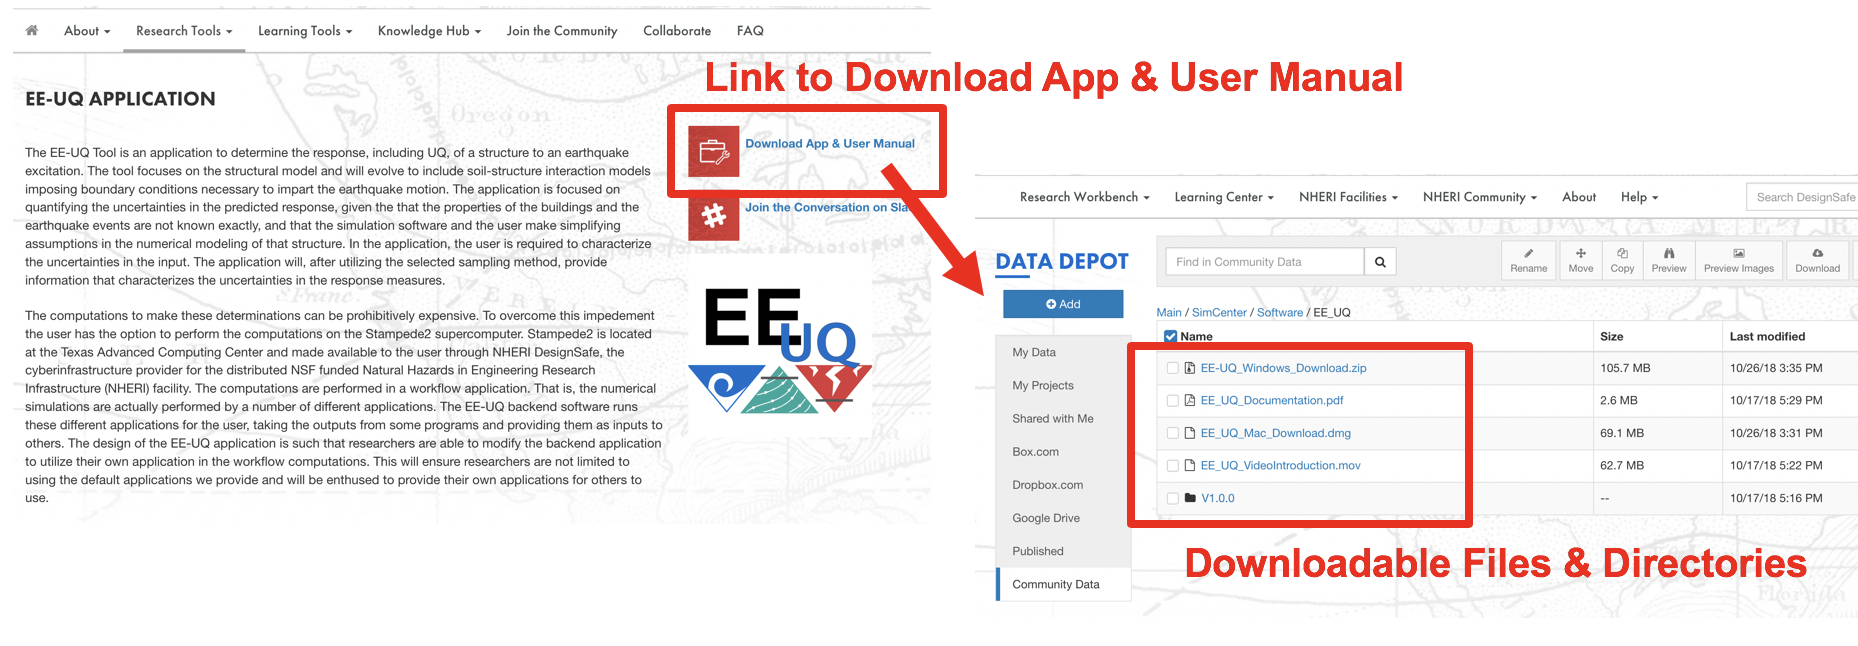
\includegraphics[width=0.95\textwidth]
    {installation/figures/eeDownload.png} }
  \caption{Download Application}
  \label{fig:app_choose_file}
\end{figure}
}{}


There are at least four files available for download from this page: 
\begin{enumerate}
    \item The PDF file is the User Manual that you are reading now.
    \item The MOV file is an video that provides an introduction to the usage of the application.
    \item The ZIP file is an archive that contains the application files for a Windows operating system.
    \item The DMG file is an archive that contains the application files for a Mac OS X operating system.
\end{enumerate}

To download the \texttt{\getsoftwarename{}} application click on the link for
the appropriate file for your operating system and then click on the
Download button at bottom right corner of the ensuing pop-up window. 
Unpackage the application from the downloaded
file and place it in a location on your filesystem. On Windows, we
recommend that you create a \texttt{C:/SimCenter/\getsoftwarename{}}
directory and extract the contents of the \texttt{ZIP} archive
there. It is also recommended to run the included installer for Visual C/C++ runtime library(vc\_redist.x64.exe). 
If you use a Mac we recommend you copy the application to either your
home folder or your Desktop folder. You are free to place the
applications anywhere you wish, you will need to make the
appropriate adjustments with the following instructions if you do so. \\

Now test that the application starts. To do this navigate to
the location where you placed the application and open it. You should
see the user interface (UI) shown in \Cref{fig:app_UI} after
starting the application. Now Quit the application. Additional steps are required before 
computations can be performed.\\

\softwareSwitch{PBE}{
\begin{figure}[!htbp]
  \centering {
    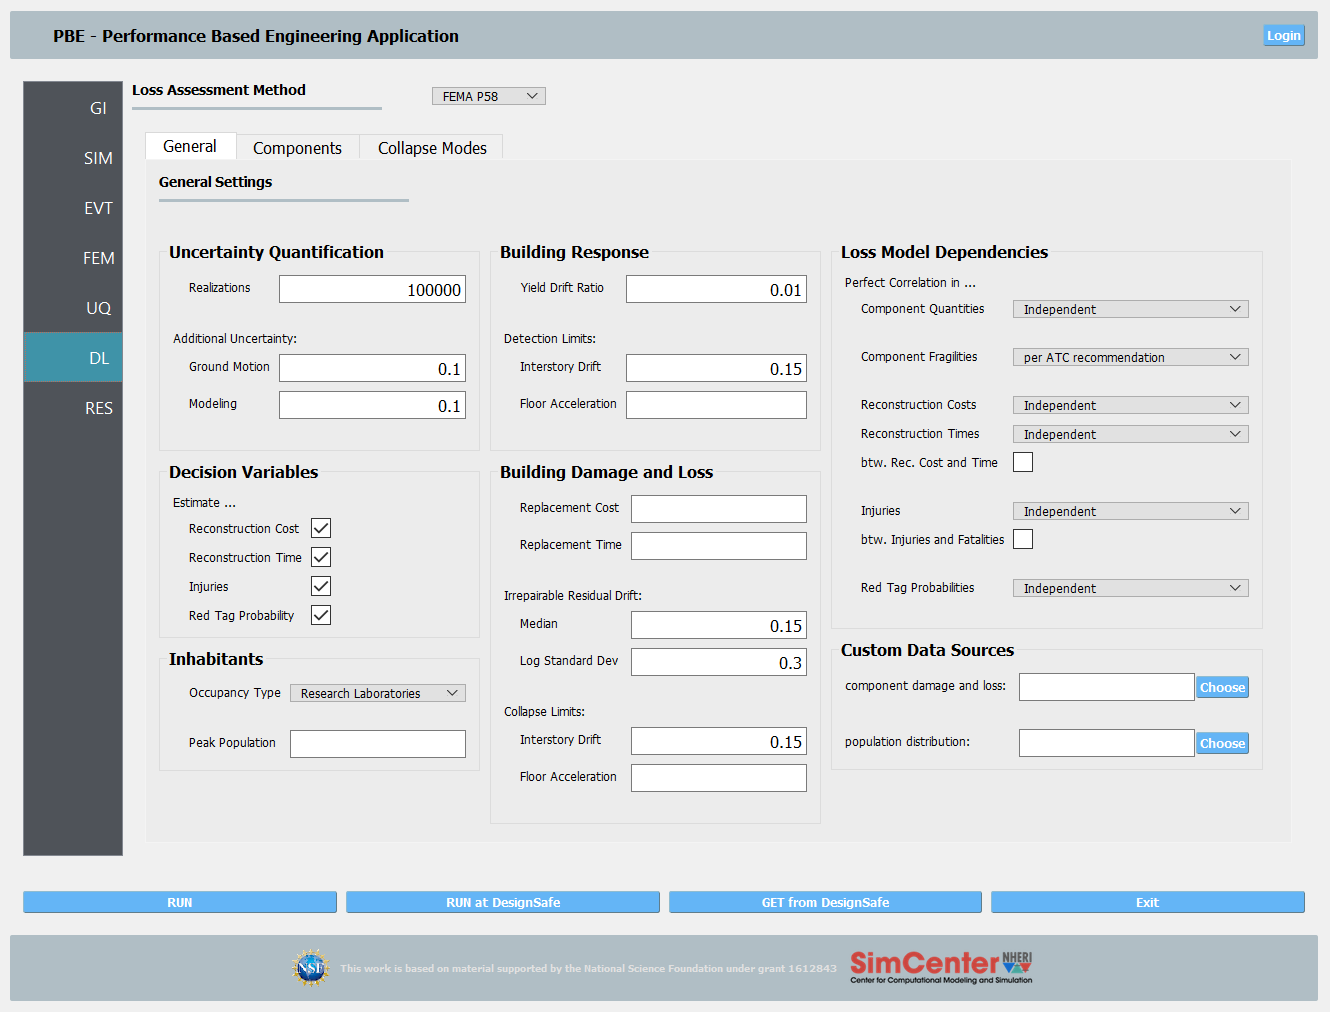
\includegraphics[width=0.95\textwidth]
    {installation/figures/PBE.png} }
  \caption{PBE Application on Startup}
  \label{fig:app_UI}
\end{figure}
}{}

\softwareSwitch{EE-UQ}{
\begin{figure}[!htbp]
  \centering {
    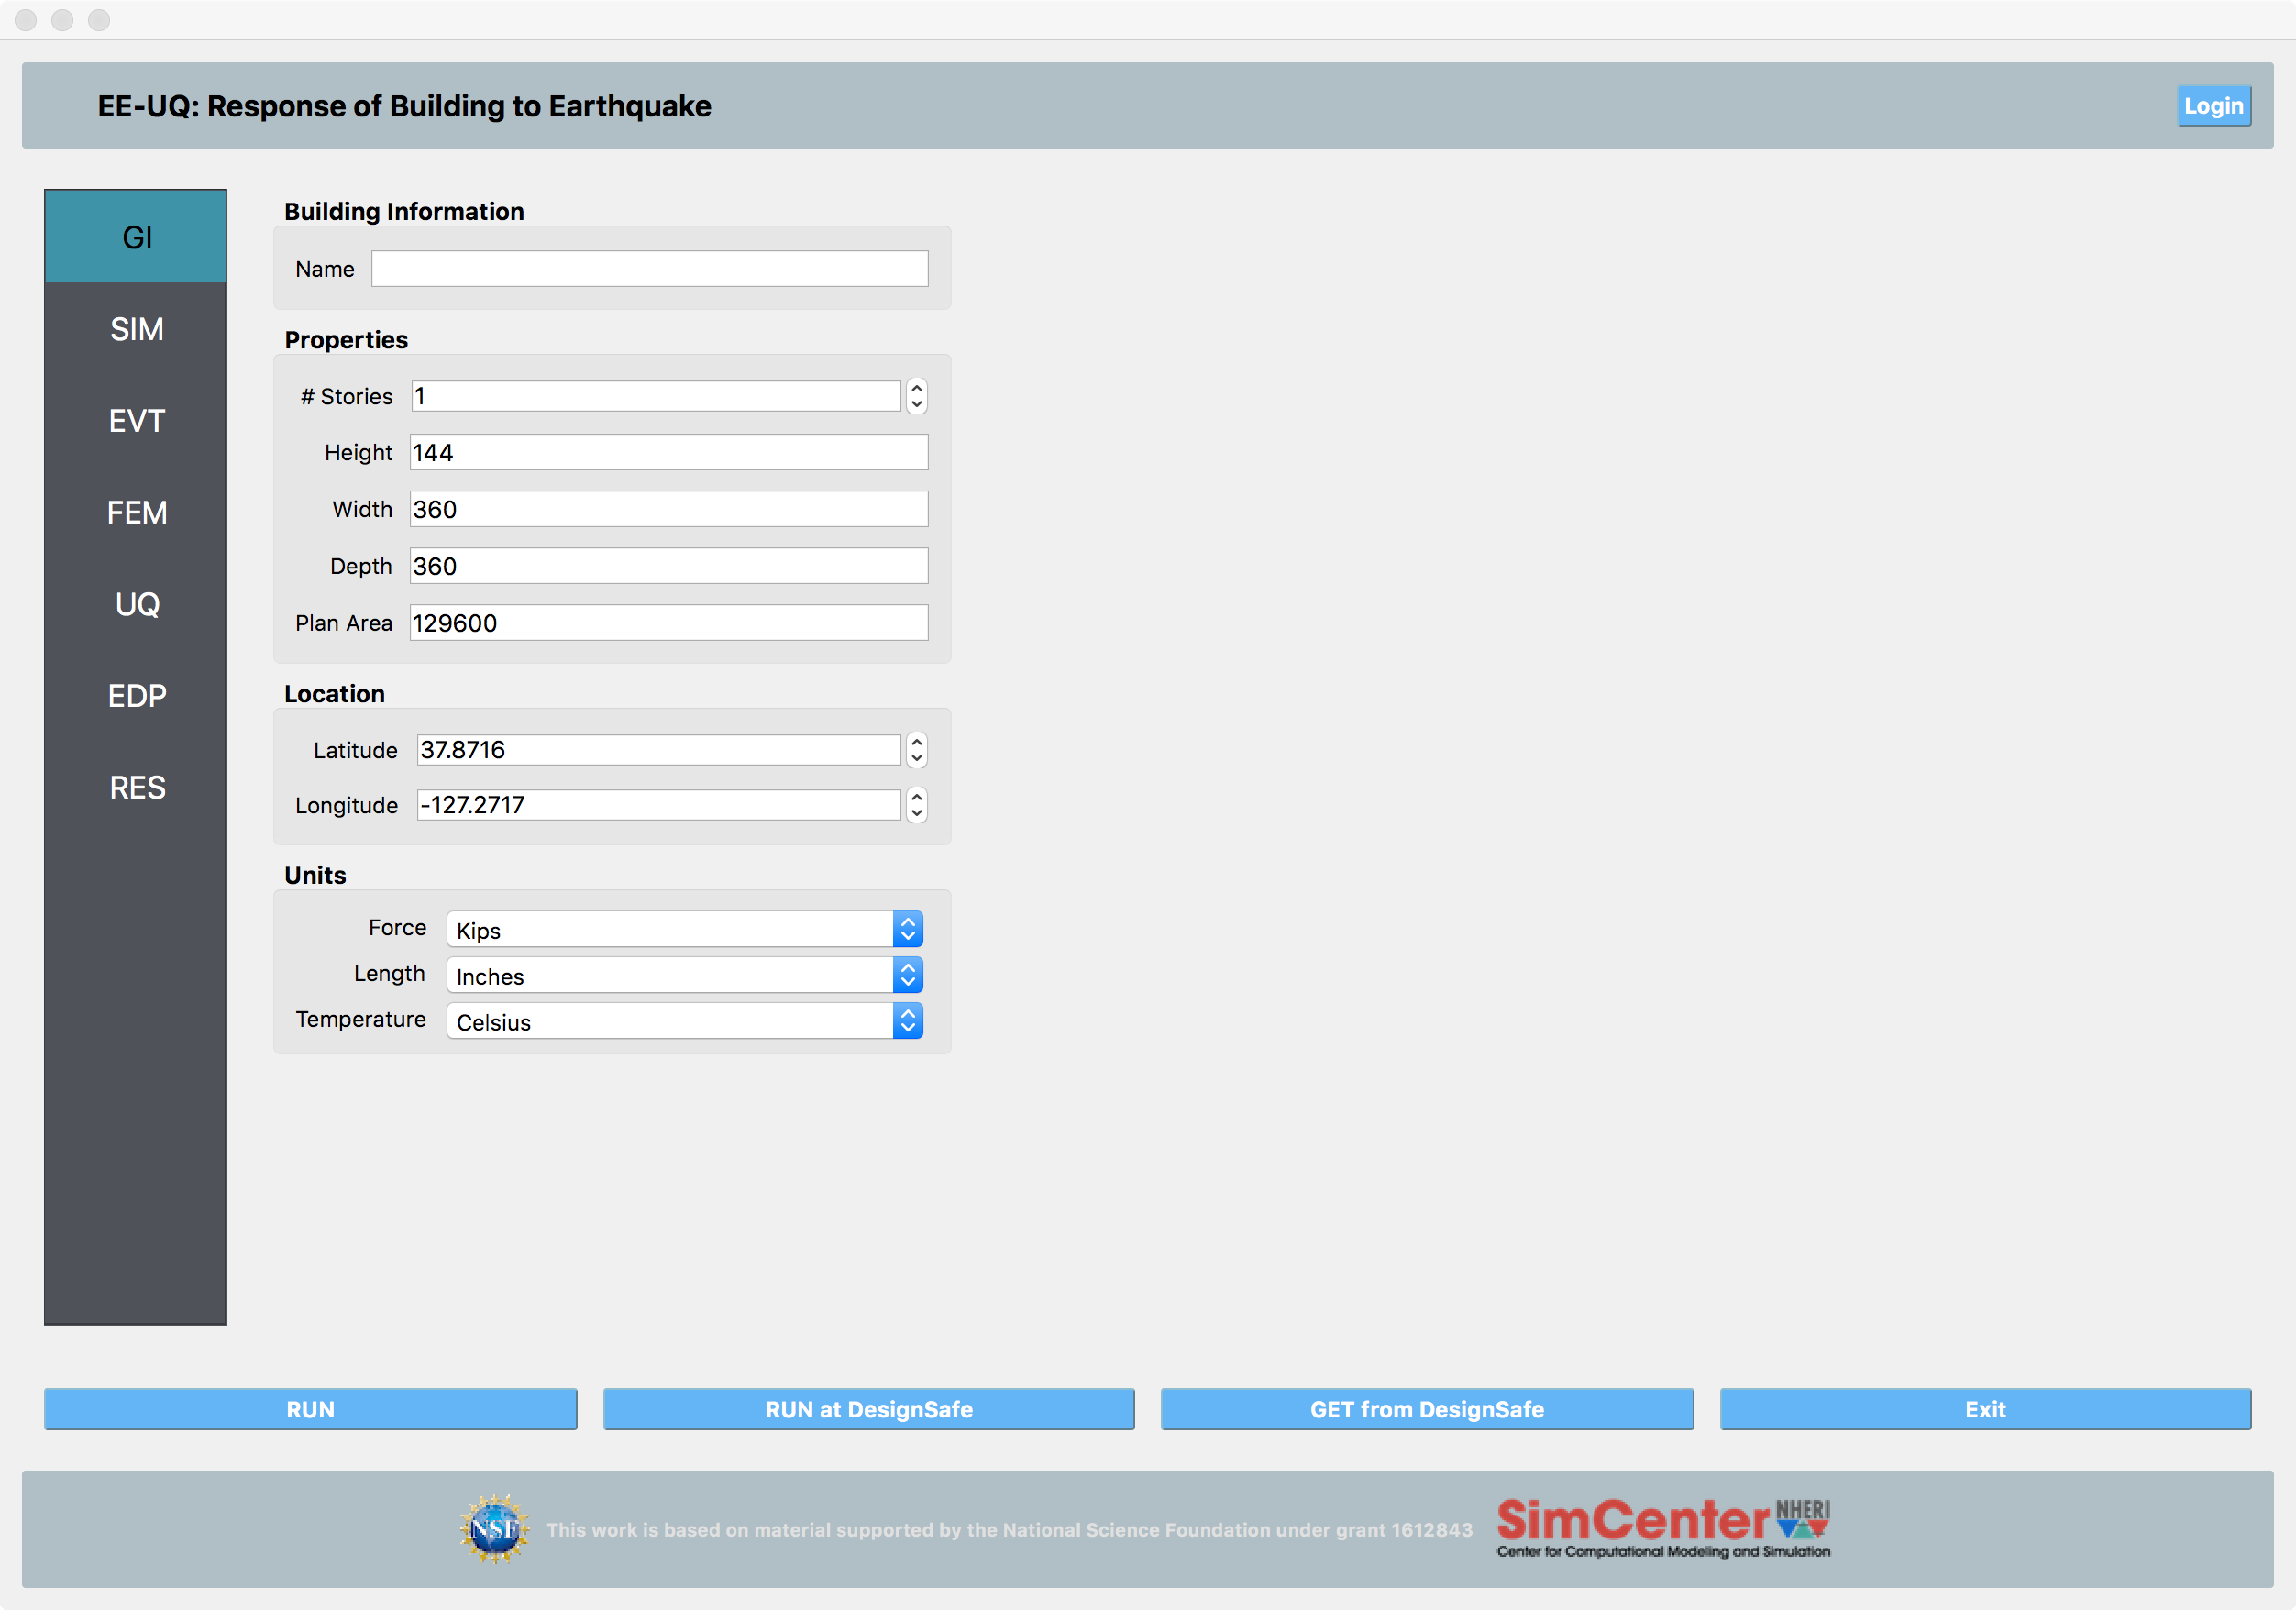
\includegraphics[width=0.95\textwidth]
    {installation/figures/EE-UQ.png} }
  \caption{EE-UQ Application on Startup}
  \label{fig:app_UI}
\end{figure}
}{}

\softwareSwitch{WE-UQ}{
\begin{figure}[!htbp]
  \centering {
    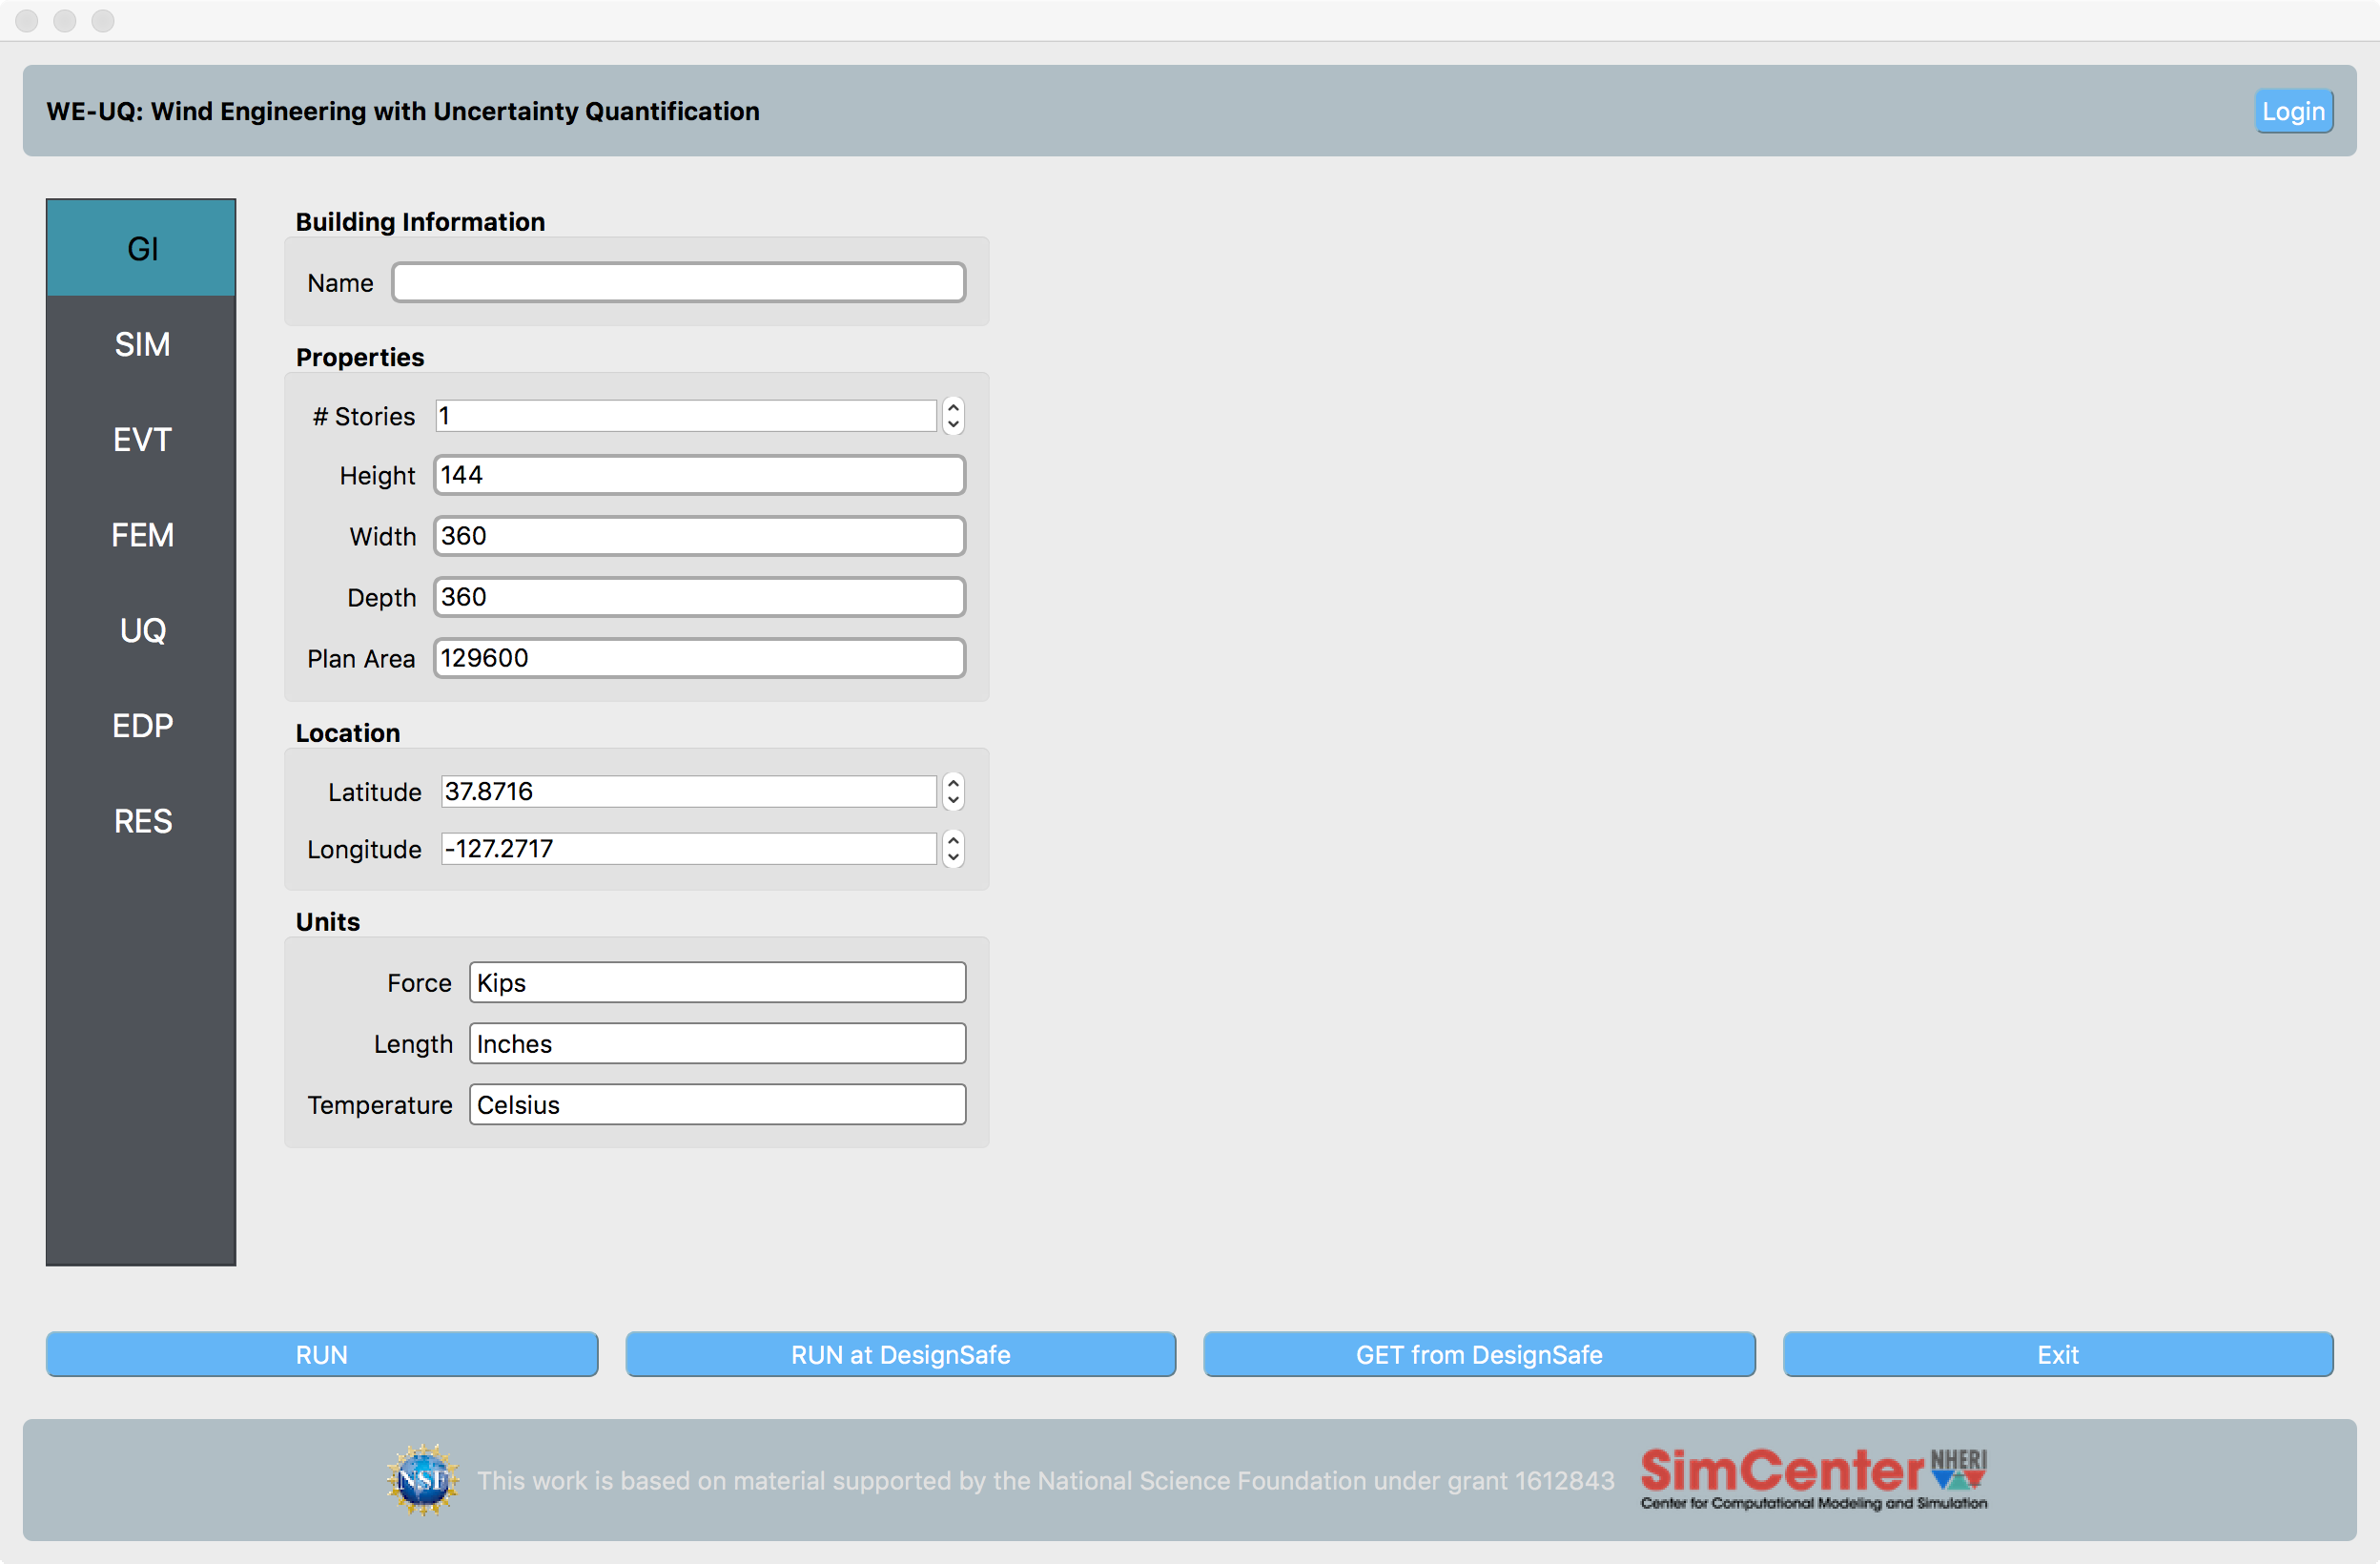
\includegraphics[width=0.95\textwidth]
    {installation/figures/WE-UQ.png} }
  \caption{WE-UQ Application on Startup}
  \label{fig:app_UI}
\end{figure}
}{}


\begin{enumerate}
\item The SimCenter is not recognized as either a Windows or an Apple vendor. Our applications are not recognized by the operating system as being signed. Consequently, you may receive a warning message when you start the \texttt{\getsoftwarename{}} application for the first time.
\item  On a Mac you will need to right click on the .dmg file to open it. The UI will not start correctly while in the DMG file, you need to open the .dmg file and then copy the \texttt{\getsoftwarename{}} application to your Documents or Desktop folder. You can then move the .dmg file to the trash or eject it after this has been done.
\item  The \texttt{\getsoftwarename{}} application requires additional software outlined in next subsections to work properly. Even of the software starts correctly, it will not run correctly until this software, outlined in the next section, is installed correctly.
\end{enumerate}


%===============================================================================
\section{Set up Python}
%===============================================================================

The SimCenter workflow applications are managed by Python
scripts. These are required to prepare the input data for running
analyses either remotely on DesignSafe or locally. As a consequence the user must have Python
installed on their machine and have the appropriate environment
variables set so that the UI can run these applications.

\subsection{Install Python}

SimCenter products require Python version 3.7 or above be installed on your machine as January 2020 marks the end of life for Python 2.7. 

\begin{enumerate}
\item Windows:

If you have not yet installed Python 3.7, we recommend installing from \href{https://www.python.org/downloads/windows}{Python.org}. We recommend installing using the \texttt{Windows x86-64 executable installer}.

Allow the installer to change your system environment variables so that the install directory is added to your PATH. Once installed you need to You need to install the following python packages: \texttt{numpy}, \texttt{scipy}, and \texttt{pandas} are installed. To install these packages open a \href{https://www.howtogeek.com/194041/how-to-open-the-command-prompt-as-administrator-in-windows-8.1/}{terminal window as an Admin user} and in that window type the following instructions:

To install these packages, start a terminal window and type:

\begin{verbatim}
pip install numpy
pip install scipy
pip install pandas
\end{verbatim}

\item Mac

The Mac comes with Python pre-installed, which is currently the somewhat 
dated version 2.7. To install Python 3.7 we recommend installing from 
\href{https://www.python.org/downloads/}{Python.org}. We recommend installing using the 
\texttt {macOS 64-bit installer} given for latest stable release. The installer will place a python3 executable in your /usr/local/bin directory, whose location should be on your system PATH.

You need to install the following python packages: \texttt{numpy}, \texttt{scipy}, and \texttt{pandas} are installed. 
To install these packages, start a terminal window and type:

\begin{verbatim}
pip3 install numpy
pip3 install scipy
pip3 install pandas
\end{verbatim}

Notes: 
\begin{enumerate}
\item To start a terminal window you can use the spotlight app (magnifying top right of desktop). Start the spotlight app and type in terminal. The terminal application should appear as the top hit. Click on it to start it.
\item In tool preferences make sure that python3 appears as the python executable. If you used older versions of SImCEnter tools this was the default.
\end{enumerate}
\end{enumerate} 

\subsection{Test Python}
%===============================================================================

Test if the python environment is set up properly by
executing \texttt{python} in a terminal window. After Python starts,
test if the packages are installed by executing \texttt{import
numpy}, \texttt{import scipy}, and \texttt{import pandas}. You will
receive an error message if a pacakage is missing. If no error
appears, the terminal should look similar
to \Cref{fig:python_test}. Exit Python by executing
the \texttt{exit()} command.

\begin{figure}[!htbp]
  \centering {
    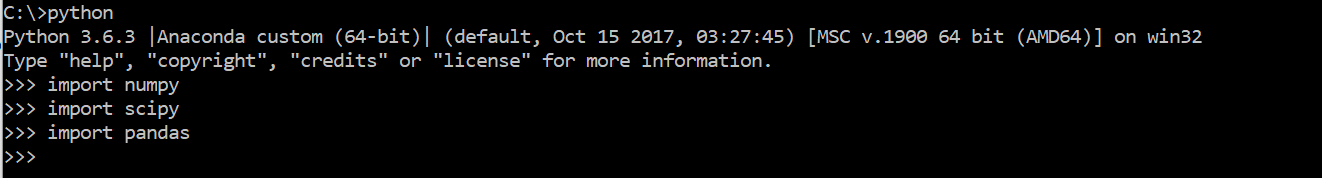
\includegraphics[width=0.8\textwidth]
    {installation/figures/python_test.png} }
  \caption{Testing the Python environment.}
  \label{fig:python_test}
\end{figure}

%===============================================================================
\section{Set up for Running Workflows Locally}\label{setup}
%===============================================================================

To run the workflows locally, the backend python application needs
publicly available software to also be installed on your
machine. These software applications need to be installed and
configured on your operating system. If you do not plan to run the
workflows locally, you will not need these applications.


\subsection{Install \texttt{OpenSees}}
%===============================================================================

\href{http://opensees.berkeley.edu}{\texttt{OpenSees}} is an open-source finite element application publicly available for download from its \href{http://opensees.berkeley.edu/OpenSees/user/download.php}{download page}. \texttt{OpenSees} installation requires the user install both \texttt{OpenSees} and \texttt{Tcl}.  If you have never downloaded \texttt{OpenSees} before, you will need to register your e-mail to gain access. After registration, you can proceed to the download page by entering your email address and clicking the Submit button. The Windows and Mac downloads are in different locations on the download page, with the appropriate Tcl installer beside the \texttt{OpenSees} link; see \Cref{fig:openseesDownload}

\begin{figure}[!htbp]
  \centering {
    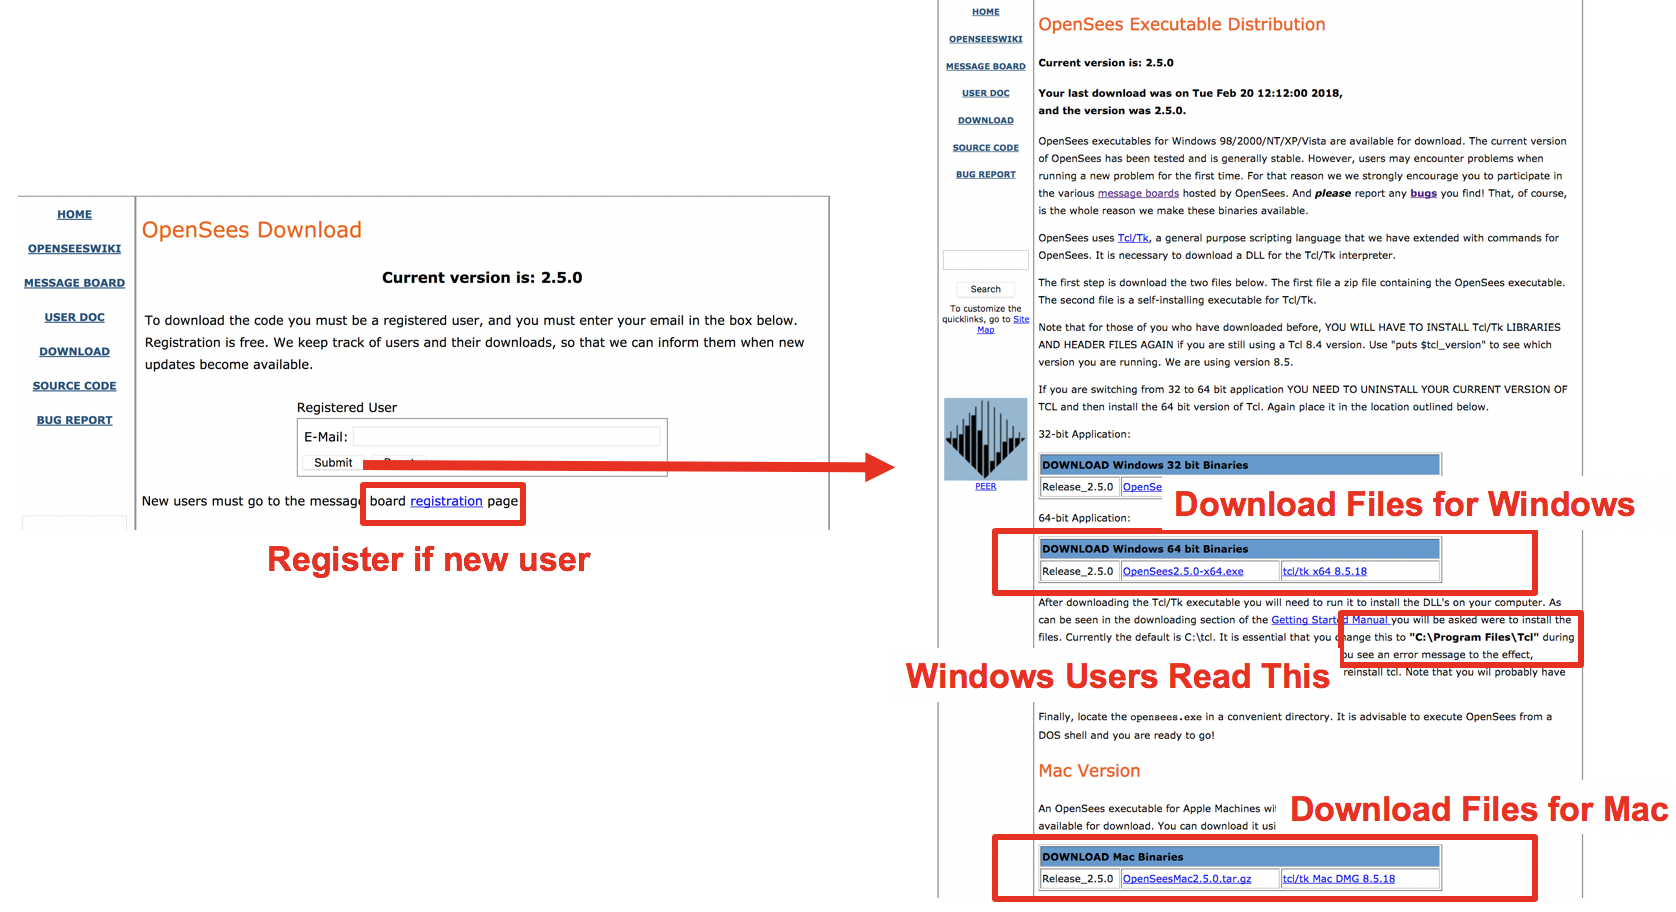
\includegraphics[width=\textwidth]
    {installation/figures/openseesDownload.png} }
  \caption{Downloading OpenSees}
  \label{fig:openseesDownload}
\end{figure}

Follow the instructions on the download page to install \texttt{Tcl}
(\Cref{fig:openseesDownload}). On Windows, you must select the Custom option for installton and you must specify
the installtion directory as \texttt{C:\textbackslash Program Files\textbackslash Tcl}, 
which is not the default. \\

After \texttt{Tcl} is installed, we recommend you put \texttt{OpenSees} in
the \texttt{C:/SimCenter/OpenSees} folder on Windows and in
a \texttt{/usr/local/OpenSees} directory on the Mac (If you use finder
on Mac to do navigation, use command-shift-G in Finder and specify
/usr/local as the folder to go to. Create a new folder \texttt{OpenSees}
and copy the \texttt{OpenSees} application to this folder).\\


Now you need to add the \texttt{OpenSees} folder to the
system \texttt{PATH} environment variable to allow the SimCenter
workflow applications to find the \texttt{OpenSees} executable on your
computer. The steps to do this depend on your operating system:

\begin{enumerate}
\item Windows: To add a folder to the \texttt{PATH} on Windows (\Cref{fig:add_env_path}):

\begin{figure}[!htbp]
  \centering {
    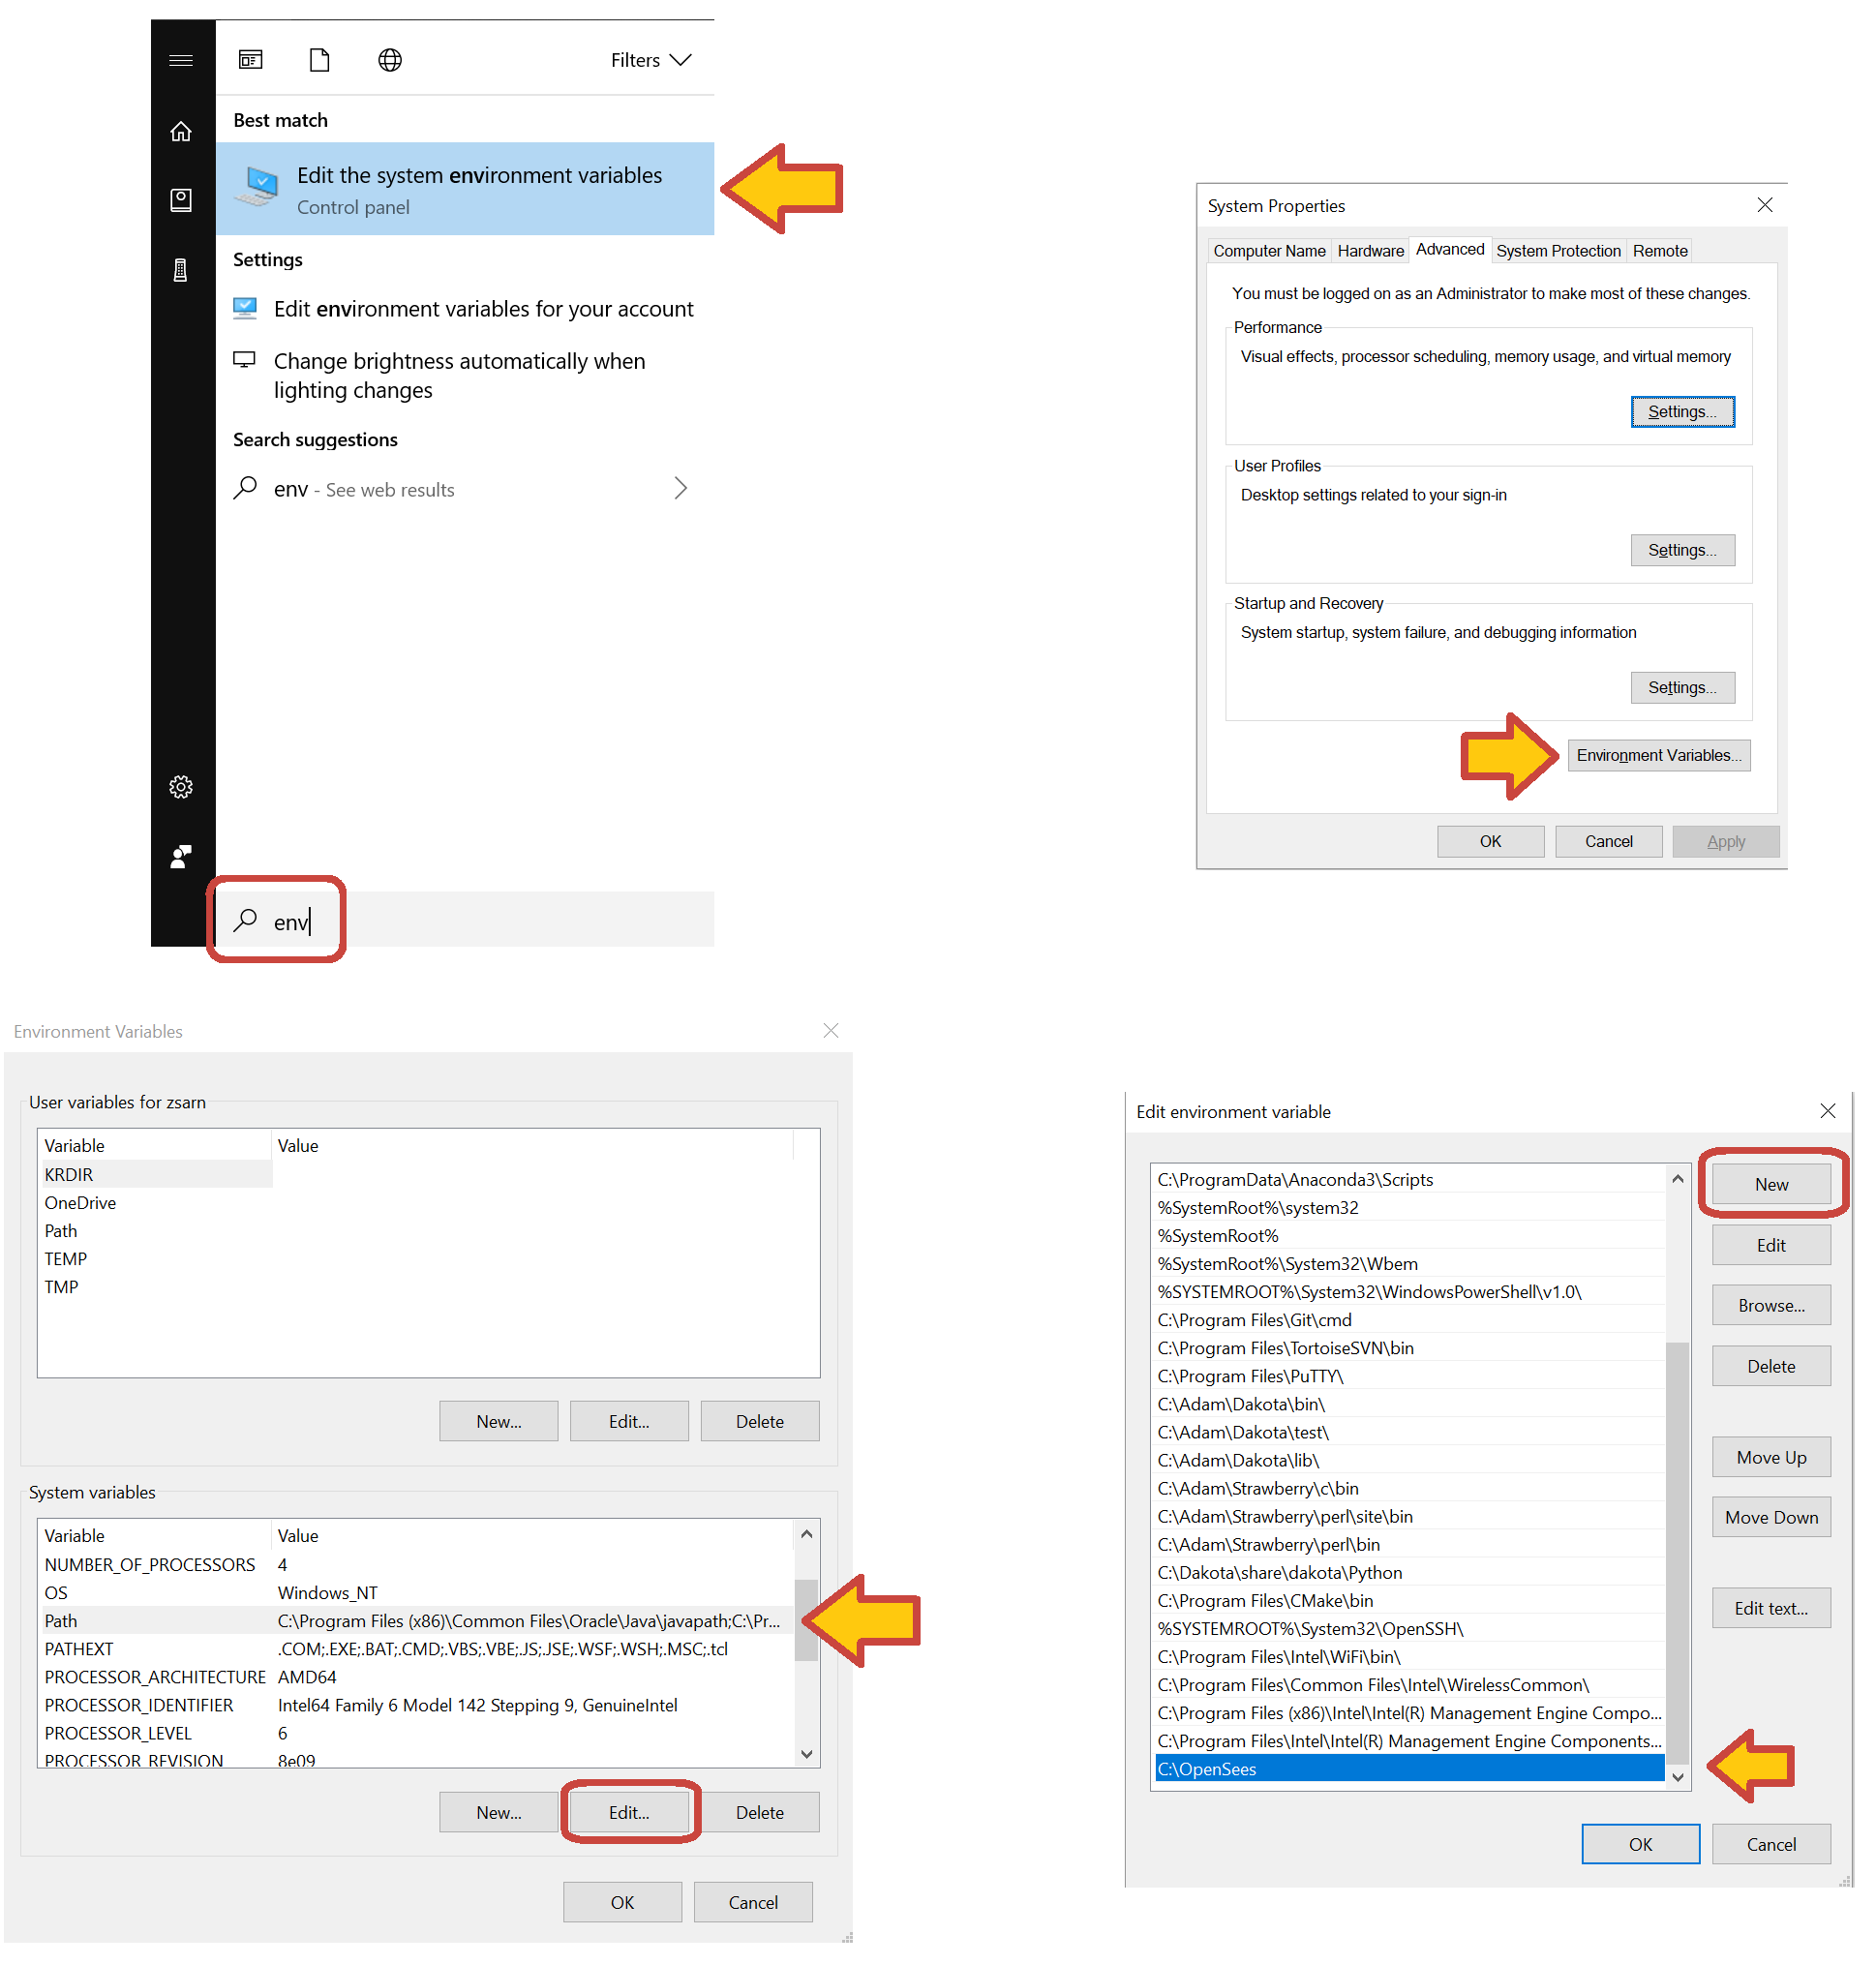
\includegraphics[width=0.8\textwidth]
    {installation/figures/add_env_path.png} }
  \caption{Adding OpenSees to the PATH environment variable on Windows}
  \label{fig:add_env_path}
\end{figure}


\begin{enumerate}
    \item open \emph{Start}, type \emph{env}, and choose \emph{Edit the system environment variables};
    \item click on the \emph{Environment variables...} button in the dialog window;
    \item find the \texttt{Path} under \emph{System Variables} in the \emph{Variable} column;
    \item click \emph{New} and type in the path to your \texttt{OpenSees.exe} (this will be \texttt{C:\textbackslash SimCenter\textbackslash OpenSees} if you put the executable at the recommended location - pay attention to using backslashes here!);
    \item click \emph{OK} in every dialog to close them and save your changes.
\end{enumerate}

\item MacOS: To add the /usr/local/OpenSees folder to the \texttt{PATH} variable:

\begin{enumerate}
    \item open a Terminal;
    \item execute (type the following in the terminal window and hit the return key) the following: \begin{verbatim}nano ${HOME}/.bash_profile\end{verbatim}
    \item if the file contains nothing, add the first 3 lines shown in \Cref{fig:add_env_path_Mac} to the file. This is done in
case an existing .bashrc file exists for your system. Adding these 3 lines will test for the existance of this file, and source in any existing commands if the file does exist.
    \item on a new line add the \texttt{OpenSees} executable to the PATH variable, by typing the following: \begin{verbatim}export PATH=/usr/local/OpenSees:${PATH}\end{verbatim}
    \item quit by hitting \texttt{Ctrl+X} and then \texttt{Y} when asked if you want to save modifications.
    \item test it is entered correctl, the following command now entered in the terminal window should result in no errors: \begin{verbatim}source ${HOME}/.bash_profile\end{verbatim}. 
\end{enumerate}

\begin{figure}[!htbp]
  \centering {
     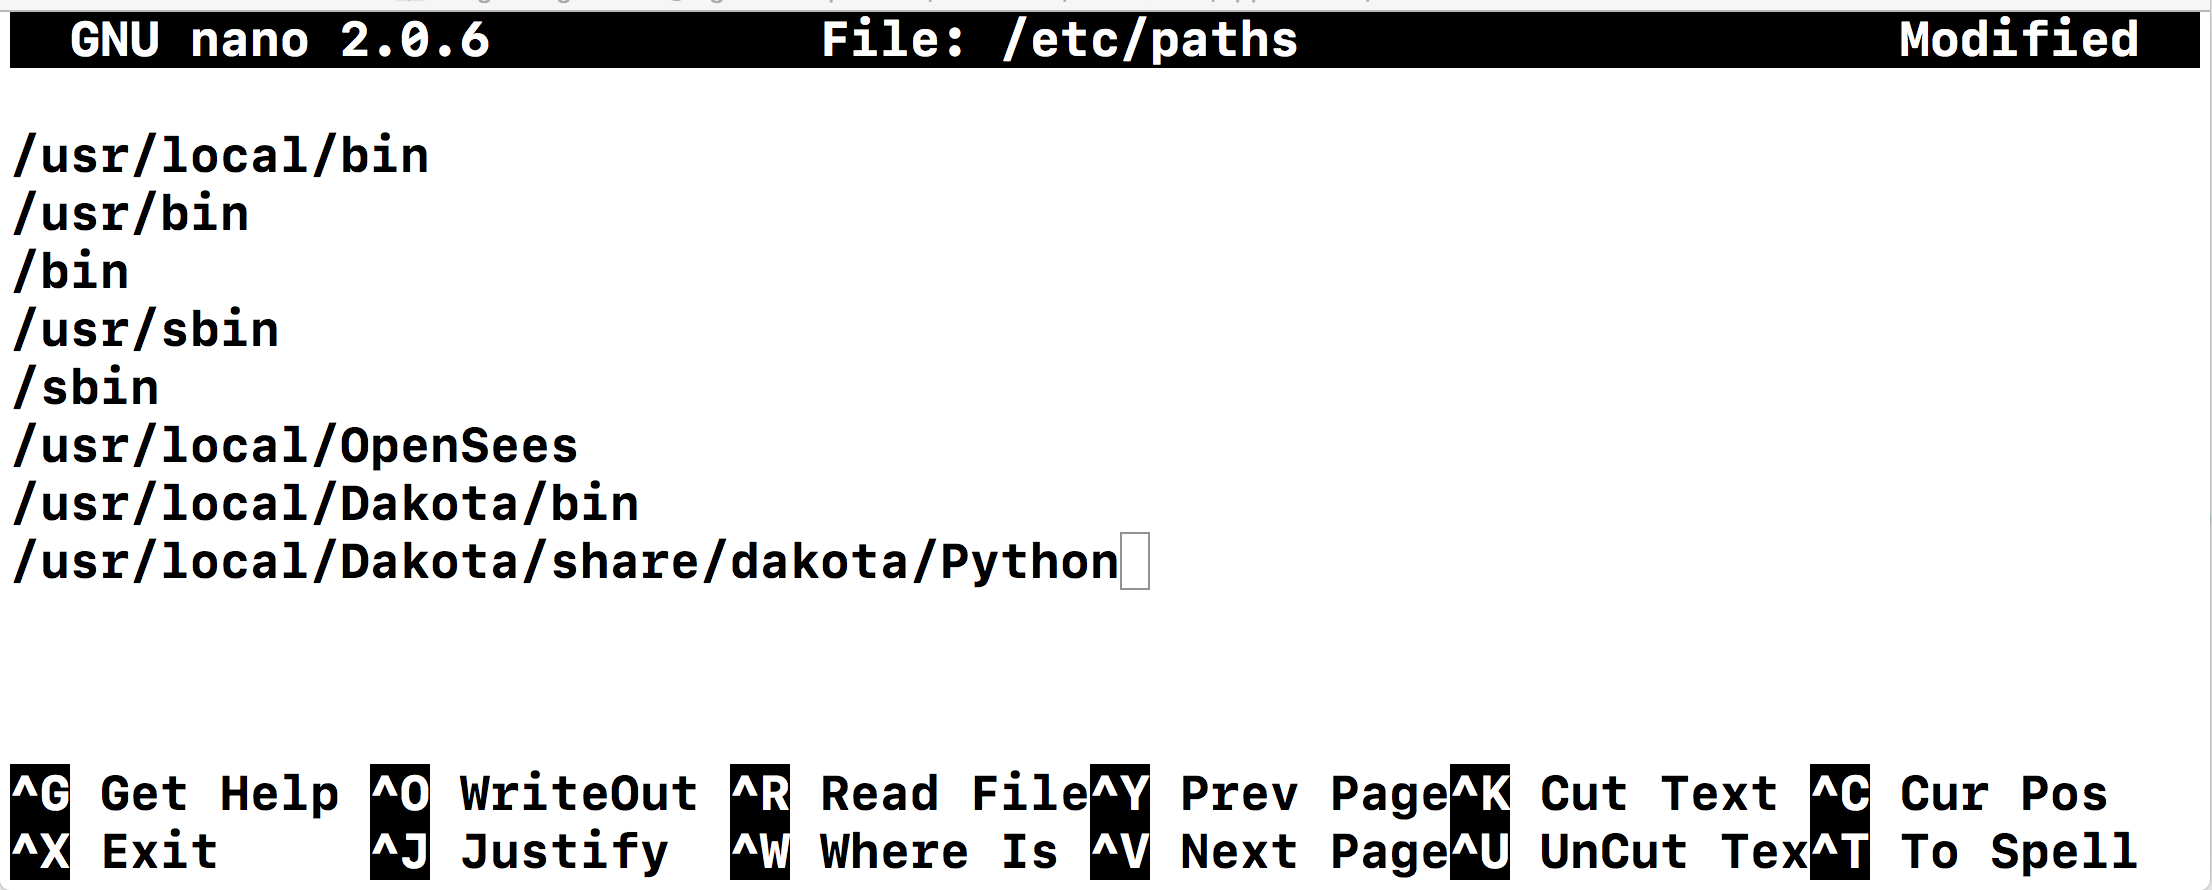
\includegraphics[width=0.8\textwidth]
    {installation/figures/add_env_path_Mac.png} }
  \caption{Adding OpenSees to the PATH environment variable on Mac.}
  \label{fig:add_env_path_Mac}
\end{figure}


\end{enumerate}


\subsection{Install \texttt{FEAPpv}}
%===============================================================================

\href{http://projects.ce.berkeley.edu/feap/feappv/}{\texttt{FEAPpv}} is a general purpose finite element analysis program which is designed for research and educational use. The program is the companion to the books: \texttt{The Finite Element Method, 7th edition, Volumes 1 and 2 (but not Vol 3)}, authored by O.C. Zienkiewicz and R.L. Taylor and published by Elsevier, Oxford, 2013.  Pre-built executables are available for download from the main \href{http://projects.ce.berkeley.edu/feap/feappv/}{web page}.


We recommend you put \texttt{FEAPpv} in
the \texttt{C:/SimCenter/FEAPpv} folder on Windows and in
a \texttt{/usr/local/FEAPpv} directory on the Mac (If you use finder
on Mac to do navigation, use command-shift-G in Finder and specify
/usr/local as the folder to go to. Create a new folder \texttt{FEAPpv}
and copy the \texttt{FEAPpv} application to this folder).\\


Now you need to add the \texttt{FEAPpv} folder to the
system \texttt{PATH} environment variable to allow the SimCenter
workflow applications to find the \texttt{FEAPpv} executable on your
computer. The steps to do this are similar to those just described for installing OpenSees.


\subsection{Install \texttt{Dakota}}
%===============================================================================

\href{http://dakota.sandia.gov}{\texttt{Dakota}}, an open-source  optimization and UQ application from Sandia National Labs, is publicly available for download at its \href{http://dakota.sandia.gov/download.html}{download page}. Select your operating system from the list and set the other options as shown in  \Cref{fig:dakota_installation}. Download the release in a \texttt{ZIP} file for Windows and \texttt{TAR.GZ} file for Mac. We recommend you to extract the archive to a \texttt{C:/SimCenter/Dakota} folder on Windows, and to a \texttt{/usr/local/Dakota} folder on a Mac.

\begin{figure}[!htbp]
  \centering {
    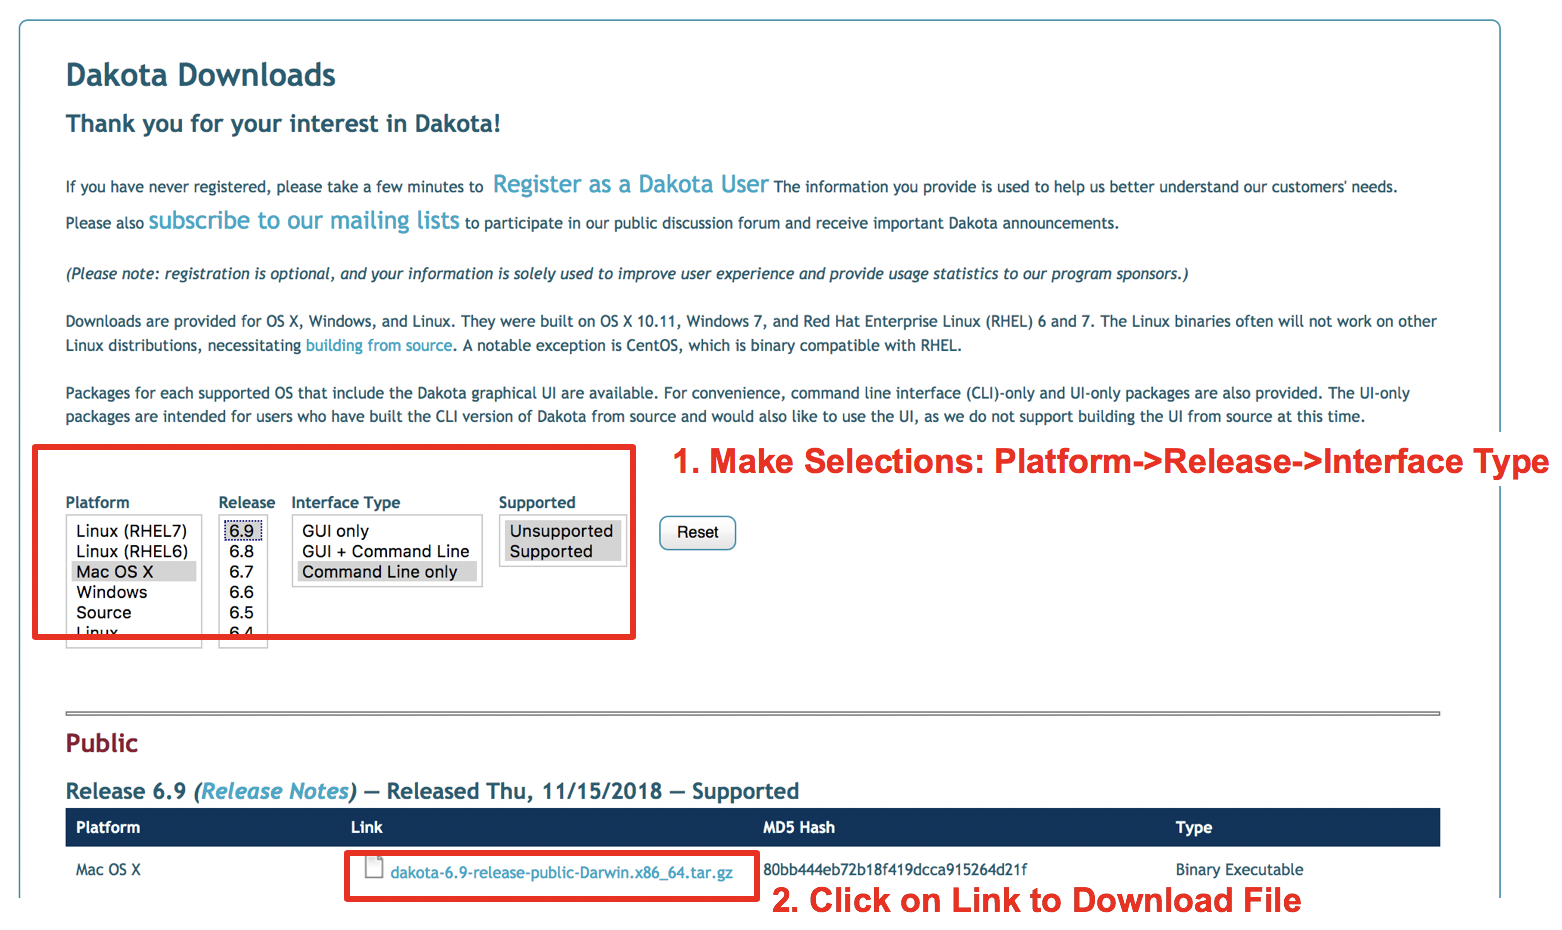
\includegraphics[width=\textwidth]
    {installation/figures/dakota_installation.png} }
  \caption{Downloading Dakota Software}
  \label{fig:dakota_installation}
\end{figure}


Following the instructions provided for installing \texttt{OpenSees}, you need to add \textbf{two} \texttt{Dakota} folders to the system \texttt{PATH} environment variable to allow the SimCenter workflow applications to find the \texttt{Dakota} tools on your computer. 
the procedure described above for \texttt{OpenSees} to add the following
folders to your \texttt{PATH}:

\begin{enumerate}
\item{Windows}

Add the following 2 folders to your windows PATH variable:
\begin{itemize}
    \item \texttt{C:\textbackslash SimCenter\textbackslash Dakota\textbackslash bin}
    \item \texttt{C:\textbackslash SimCenter\textbackslash Dakota\textbackslash share\textbackslash dakota\textbackslash Python}
\end{itemize}

Now you need to create a new variable, \texttt{PYTHONPATH}, and point it to the following folder.


\begin{itemize}
    \item \texttt{C:\textbackslash SimCenter\textbackslash Dakota\textbackslash share\textbackslash dakota\textbackslash Python}
\end{itemize}

\item{MacOS}
On the Mac you also need to add 2 lines, previously shown in \Cref{fig:add_env_path_Mac},
 to the .bash\_profile file. One line adds the Dakota executable to the PATH variablem and 
the other creates a new variable PYTHONPATH and points it to a folder in the  Dakota 
installation directory. 

\begin{itemize}
    \item \texttt{export PATH=/usr/local/Dakota/bin:\${PATH}}
    \item \texttt{export PYTHONPATH=/usr/local/Dakota/share/dakota/Python}
\end{itemize}
\end{enumerate}


\subsection{Test the Install of the Local Applications}
%===============================================================================

Before running the \texttt{\getsoftwarename{}} application, perform the following tests to
make sure that the local SimCenter working environment is set up
appropriately:

\begin{itemize}
    \item Start a Terminal on Mac or a Command Prompt on Windows.
    \item On Mac, execute \texttt{cd /usr/Documents} to change the active directory to \texttt{/usr/Documents}. On Windows, execute \texttt{cd C:/} to change the active directory to \texttt{C:/}.
    \item Test if \texttt{OpenSees} works correctly by executing the \texttt{OpenSees} command. The command should start \texttt{OpenSees} (\Cref{fig:opensees_test}). Close \texttt{OpenSees} with the \texttt{exit} command.
    \item Test if \texttt{Dakota} works correctly by executing the \texttt{dakota} command. The command should start \texttt{Dakota} and you should see a message about a missing argument (\Cref{fig:dakota_test}).
    \item Test if the python package in \texttt{Dakota} works correctly by starting Python with the \texttt{python} command and then executing the \texttt{import dakota} command. This should import the dakota package. If you do not see errors, then the package is successfully imported (\Cref{fig:dakota_py_test}). Exit Python with the \texttt{exit()} command.
    \item If all the above tests ran without errors, your environment is set up appropriately.
\end{itemize}

\begin{figure}[!htbp]
  \centering {
    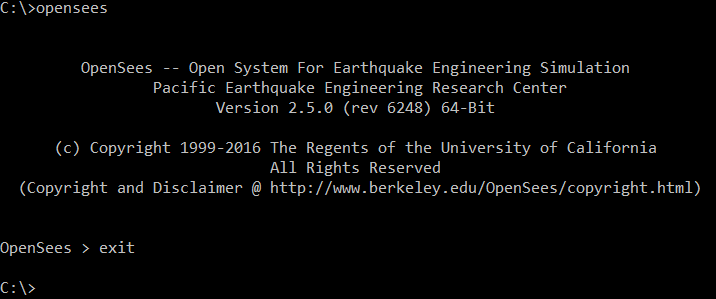
\includegraphics[width=0.8\textwidth]
    {installation/figures/opensees_test.png} }
  \caption{Testing OpenSees.}
  \label{fig:opensees_test}
\end{figure}

\begin{figure}[!htbp]
  \centering {
    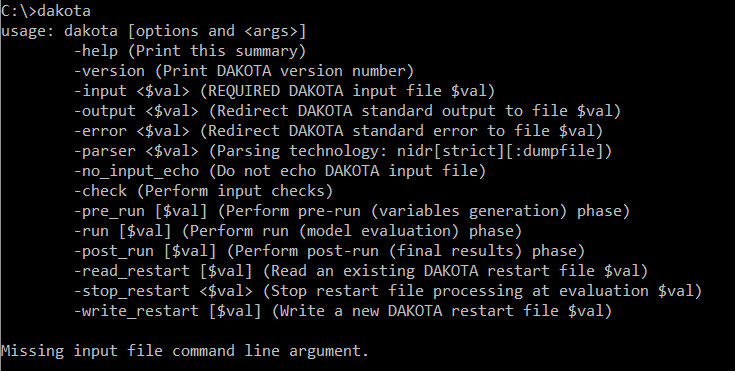
\includegraphics[width=0.8\textwidth]
    {installation/figures/dakota_test.png} }
  \caption{Testing Dakota.}
  \label{fig:dakota_test}
\end{figure}

\begin{figure}[!htbp]
  \centering {
    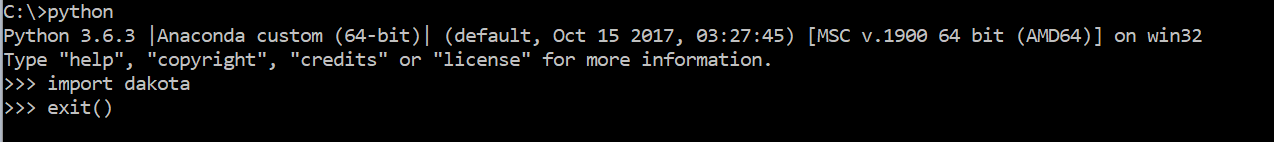
\includegraphics[width=0.8\textwidth]
    {installation/figures/dakota_py_test.png} }
  \caption{Testing the dakota Python package.}
  \label{fig:dakota_py_test}
\end{figure}



\chapter{Usage}
\label{chap:usage}
\section{User Interface}
The user interface (UI), as shown in \Cref{fig:generic_ui}, is where the analysis
is configured and managed. Here, the user is able to provide the necessary
parameters to create the simulation, start the simulation both locally and
remotely, and view the simulation results. The interface contains several
separate areas:

\begin{figure}[!htbp]
  \centering {
    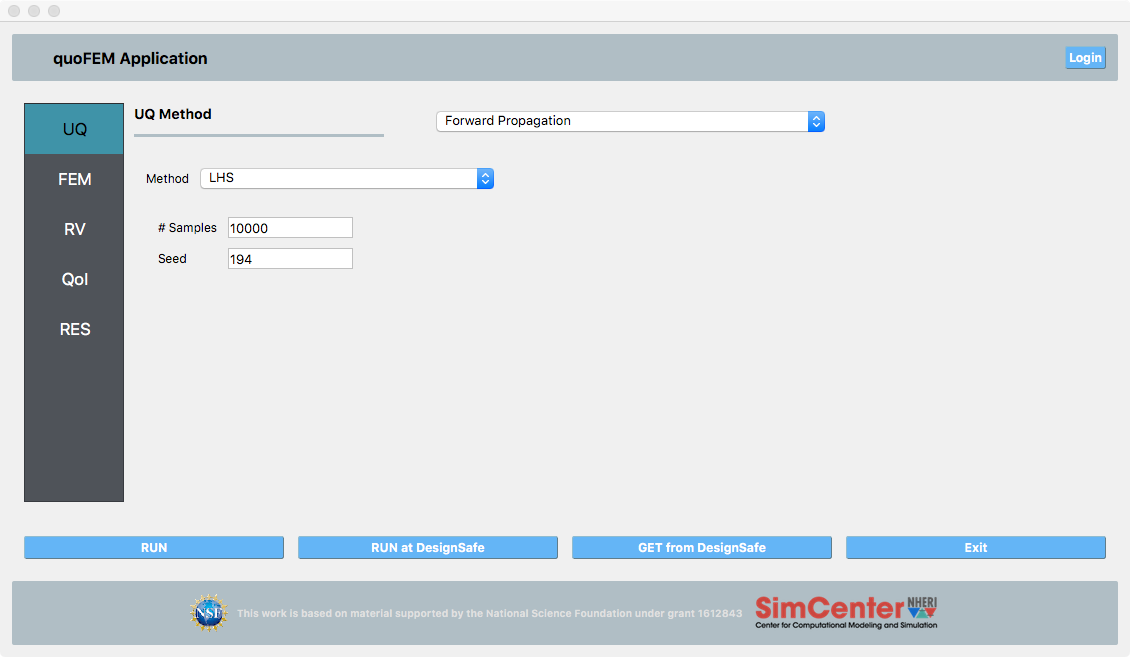
\includegraphics[width=0.95\textwidth]
    {examples/fig_quofem/fw.png} }
  \caption{The User Interface (UI)}
  \label{fig:generic_ui}
\end{figure}

\begin{enumerate}
\item Input Panel Selection: This area on the left side provides the
  user with a selection of items to choose from:
\begin{enumerate}
  \item UQ: the input panel for specifying everything related to Uncertainty Quantification analysis.
  \item FEM: the input panel for Finite Element model specification.
  \item RV: the input panel for the specification of random input for the problem at hand.
  \item QoI: the input panel for specifying the desired output to extract from each Finite Element simulation.
  \item RES: results tab for outputting all tables, figures, results, graphs, from the quoFEM application.  
\end{enumerate}

Selecting any of these will change the input panel presented.

\item Push Buttons: This is the area near the bottom of the UI in
  which 4 buttons are presented to the user:

\begin{enumerate}
\item RUN – Run the simulation locally on the user’s desktop machine.
\item RUN at DesignSafe – Process the information, and send to
  DesignSafe. The simulation will be run there on a supercomputer, and results
  will be stored in the user's DesignSafe jobs folder.
\item GET from DesignSafe – Obtain the list of
  jobs for the user from DesignSafe and select a job to download from that list.
\item Exit: Exit the application.
\end{enumerate}

The first 3 of the above buttons and their use are discussed in more detail in \Cref{sec:push_buttons}.

\item Login Button: The Login Button is at the top right of the UI. Before the user can launch any jobs on DesignSafe, they must
  first login to DesignSafe using their DesignSafe login and
  password. Pressing the login button will open up the login window
  for users to enter this information. Users can register for an
  account on
  the \href{https://www.designsafe-ci.org/account/register/}{DesignSafe
  webpage}.

\item Message Area: While the application is running, error and status messages will be displayed here, in the top center of the user interface.

\end{enumerate}


\section{UQ: Uncertainty Quantification}
\label{sec:uq}
Throughout the input specification the user is defining variables. As
described in the above sections many of these variables can be
specified by the user to be random variables. The UQ panel is where the user specifies the distribution of these random variables. Besides the properties of random variables, the sampling method and the number of requested samples shall also be defined by the user. The panel is split, as shown
in \Cref{fig:uq_panel}, into two frames:

\begin{enumerate}
\item Sampling Methods 
\item Random Variables
\end{enumerate}

\begin{figure}[!htbp]
  \centering {
    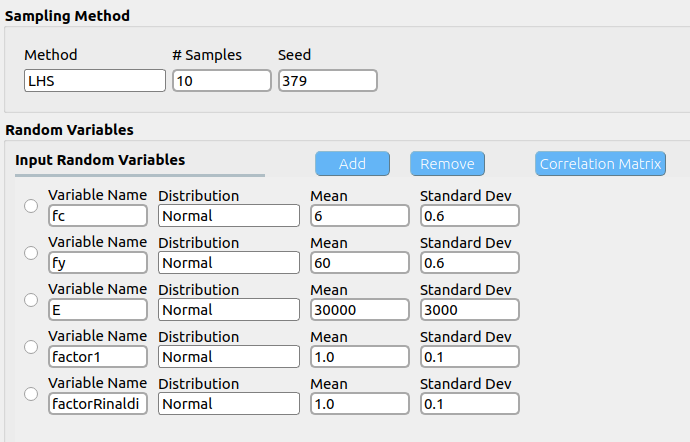
\includegraphics[width=0.8\textwidth]
    {usage/figures/uq1.png} }
  \caption{Uncertainty Quantification input panel}
  \label{fig:uq_panel}
\end{figure}

\subsection{Sampling Methods}
In the \href{https://dakota.sandia.gov//sites/default/files/docs/6.9/html-ref/method-sampling.html}{sampling methods} the user selects the sampling 
method to use from the dropdown menu. Currently there are two options available: 
Monte Carlo and Latin Hypercube Sampling (LHS). Depending on the option selected, the user must specifies the number of samples and the seed. The number of samples specifies the number of simulations to be performed. Providing a random seed allows the user to reproduce the same set of samples from the random variables multiple times.

\subsection{Random Variables}
The Random Variable panel allows the user to characterize the random
variables. Each random variable has a name and a distribution. The
distribution is selected from the drop-down menu. By changing the
distribution type, the parameters required to define the distribution
change. The following distributions are available (clicking on a link will take you to the Dakota manual that provides theoretical background and explains the requested parameters for each distribution):
\begin{enumerate}
\item \href{https://dakota.sandia.gov//sites/default/files/docs/6.9/html-ref/variables-normal_uncertain.html}{Normal}
\item \href{https://dakota.sandia.gov//sites/default/files/docs/6.9/html-ref/variables-lognormal_uncertain.html}{Lognormal}
\item \href{https://dakota.sandia.gov//sites/default/files/docs/6.9/html-ref/variables-beta_uncertain.html}{Beta}
\item \href{https://dakota.sandia.gov//sites/default/files/docs/6.9/html-ref/variables-uniform_uncertain.html}{Uniform}
\item \href{https://dakota.sandia.gov//sites/default/files/docs/6.9/html-ref/variables-weibull_uncertain.html}{Weibull}
\item \href{https://dakota.sandia.gov//sites/default/files/docs/6.9/html-ref/variables-gumbel_uncertain.html}{Gumbel}
\end{enumerate} 

As with other panels, the random variables can be added or
removed. Care must be taken by the user in ensuring that if the user
removes random variables from this panel that they also remove them
from the other input widgets. Failing to do so may result in the
program failing to complete.


\section{FEM: Finite Element Method}
\label{sec:fem}
The FEM panel will present users with a selection of FEM
applications. Currently, there is two application
available, OpenSees and FEAPpv. More FE platforms will be added 
 in future versions to allow users to provide their own
simulation application.  

\begin{figure}[!htbp]
  \centering {
    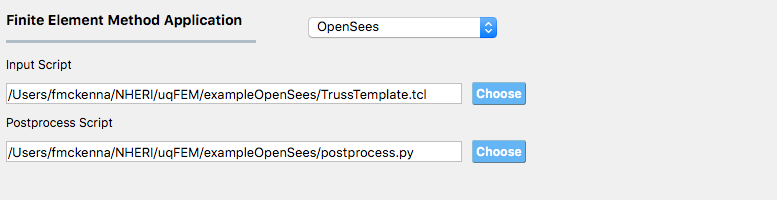
\includegraphics[width=0.8\textwidth]
    {examples/fig_quofem/fem.png} }
  \caption{Options for FEM file specification with OpenSees}
  \label{fig:fem}
\end{figure}

\begin{figure}[!htbp]
  \centering {
    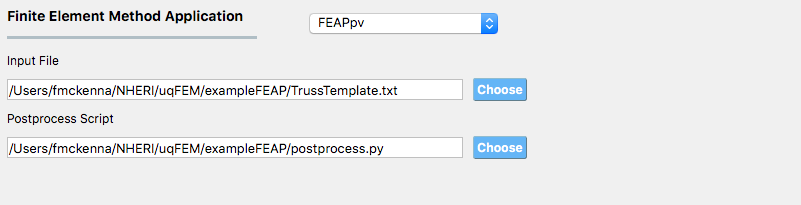
\includegraphics[width=0.8\textwidth]
    {examples/fig_quofem/fem2.png} }
  \caption{Options for FEM file specification with FEAPpv}
  \label{fig:fem2}
\end{figure}

For the OpenSees and FEAPpv applications, the user is required to specify the FEM input file, as shown in \Cref{fig:fem} and \Cref{fig:fem2}, respectively. A user-provided post-processing script for each FEM application needs to be selected appropriately. 

\section{RV: Random Variables}
\label{sec:rv_quofem}
The RV panel allows the user to specify the probabilistic distribution for the random problem at hand. The following probabilistic distributions for the random variables are currently supported: 
\begin{enumerate}
\item Gaussian
\item Lognormal
\item Beta
\item Uniform
\item Weibull
\item Gumbell
\end{enumerate}

Each distribution has different parameters, and the user needs to select accordingly the parameters for the distribution selected for each random variable. Once the user selects the distribution of the random variable, the
corresponding input boxes for the parameters will show. 

\Cref{fig:rv} shows the panel for a problem with four Random Variables with all random input following Gaussian distributions. 

\begin{figure}[!htbp]
  \centering {
    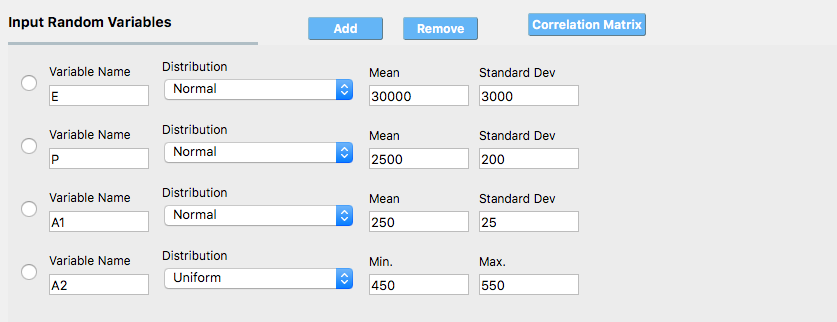
\includegraphics[width=0.8\textwidth]
    {examples/fig_quofem/rv.png} }
  \caption{Random Variable specification}
  \label{fig:rv}
\end{figure}




\section{QoI: Output}
\label{sec:qoi_quofem}
The QoI panel provide the user the capability to specify the output of the FEM results. The user needs to specify the name tag associated with the random output of the FEM simulation to which uncertainty results need to be produced. 

\section{RES: Results}
\label{sec:res_quofem}
A successful run or download of a job that ran successfully will result in 3 tabbed
widgets being displayed in the results panel.  The first tab, as shown in
\Cref{fig:results_summary}m shows summary statistics: mean and
stdDev values or min-max values (if discrete set is used to define one or more of the random variables, e.g multiple events)
are shown for each of the EDP's specified. The second panel,
shown in \Cref{fig:summary_information} shows the summary
information from Dakota output file containing other statstics generated by Dakota.

\begin{figure}[!htbp]
  \centering {
    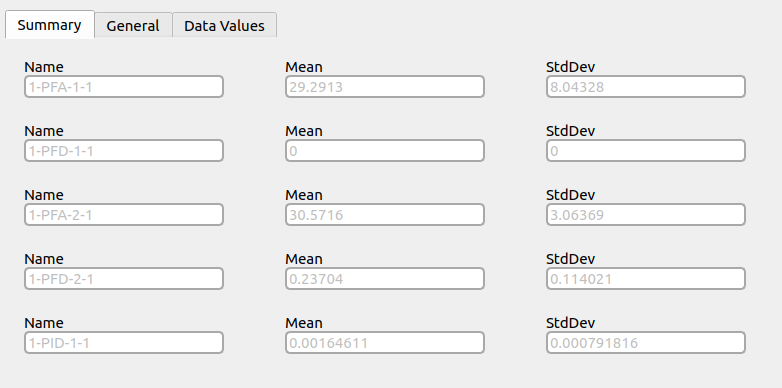
\includegraphics[width=0.8\textwidth]
    {usage/figures/resultsSummary.png} }
  \caption{Results Summary}
  \label{fig:results_summary}
\end{figure}

\begin{figure}[!htbp]
  \centering {
    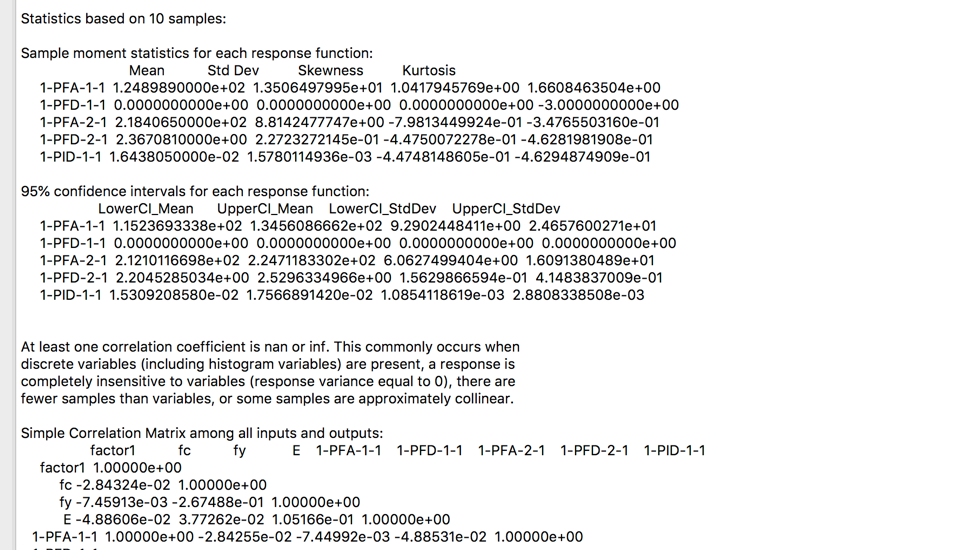
\includegraphics[width=0.8\textwidth]
    {usage/figures/resultsInformation.png} }
  \caption{\texttt{General} tab showing results summary information}
  \label{fig:summary_information}
\end{figure}

The third panel, shown in \Cref{fig:results_data} presents the results both
graphically and in tabular form. By selecting different
columns with left and right mouse buttons in the table below the
graphic, the information in the graph is changed. Selecting the left
mouse button changes the Y axis, the right mouse changes the X
axis. If the same column is selected using both left and right keys,
either the CDF and PDF is displayed. If the last mouse press was with the left
button, the PDF will be displayed; if the last mouse press was the right one, the CDF
will be displayed.
 
Regarding the columns in the table below the figure: You will see a column for each random variable the workflow came across and then the columns for the response quantaties. There may be more random variables than you specified. This is because certain applications the user selected may introduce additional random varaibles for the UQ engine to consider. 

\begin{figure}[!htbp]
  \centering {
    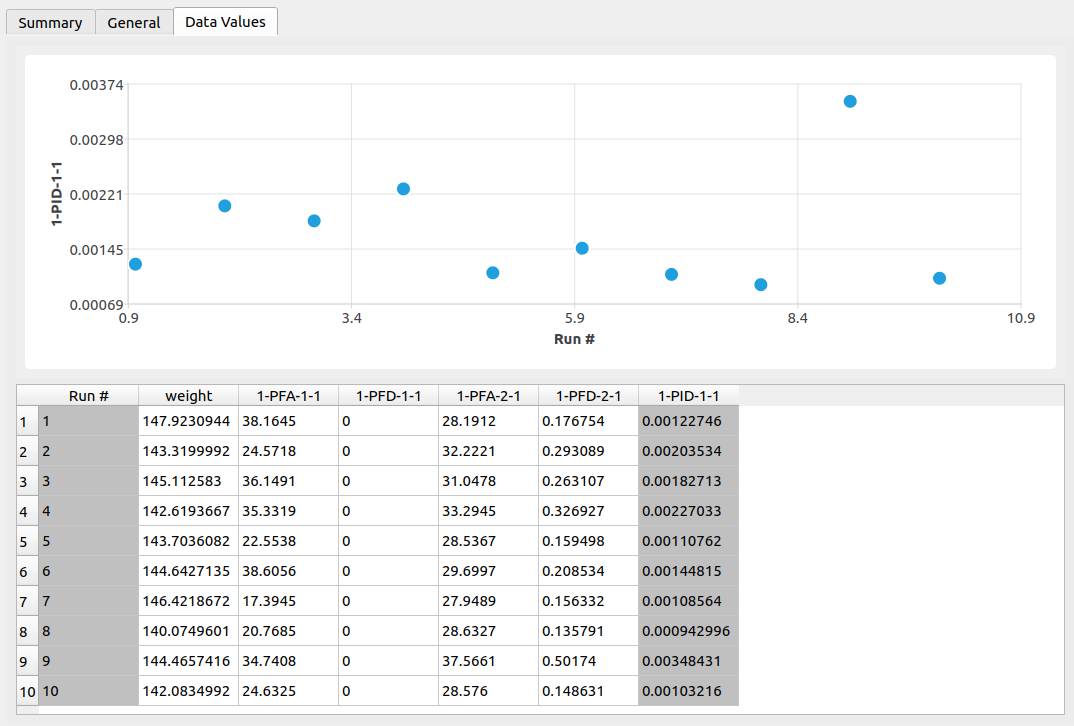
\includegraphics[width=0.8\textwidth]
    {usage/figures/resultsData.png} }
  \caption{Results presented graphically and in tabular form}
  \label{fig:results_data}
\end{figure}



\chapter{Verification and Validation}
\label{chap:vnv}
This chapter provides examples of using the \texttt{\getsoftwarename{}} application for uncertainty
quantification of Finite Element models. Results of each model are verified against results
obtained using other tools. 
\\

\section{Two-Dimensional Truss Structure}
Consider the problem of uncertainty quantification in a two-dimensional truss structure, as shown in figure \Cref{fig:truss}. 

The structure has uncertain properties that all follow normal distribution such that:
\begin{enumerate}
\item Elastic moduli: $\bar{E}=205kN/mm^2$, and $\sigma_{E}=15 kN/mm^2$ 
\item Load: $\bar{P}=25kN$, $\sigma_{P}=2.5kN$
\item Cross sectional area for the upper three bars: $A_u=500mm^2$, and $\sigma_{A_u}=25mm^2$
\item  Cross sectional area for the other six bars: $A_l=250mm^2$, and $\sigma_{A_l}=10mm^2$
\end{enumerate}

Table \Cref{tab:uncertainty} summarizes the uncertain input mentioned above. 

\begin{figure}[!htbp]
  \centering {
    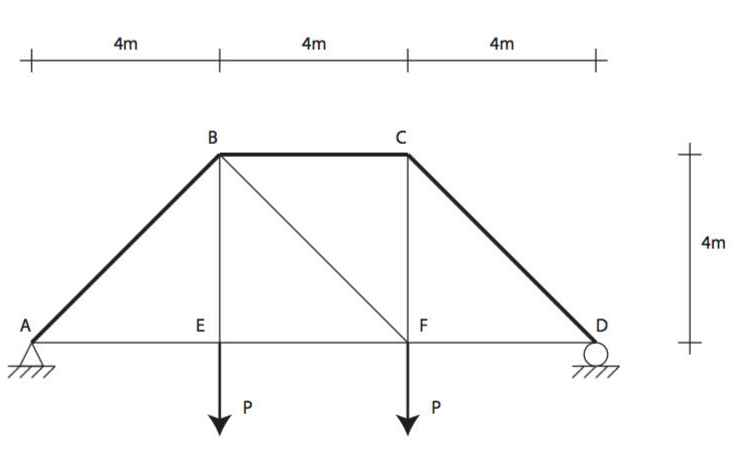
\includegraphics[width=0.8\textwidth]
    {examples/fig_quofem/truss.png} }
  \caption{Two-dimensional truss model used in Verification.}
  \label{fig:truss}
\end{figure}

\begin{table}[hbt!]                       
  \centering
\begin{adjustbox}{max width=\textwidth}            
  \begin{tabular}{lllll}                    
    \toprule          
      Uncertain Parameter & 	Distribution	 &  Mean  &  Standard Deviation \\ \hline
	Elastic Moduli $[kN/mm^2]$	 & Normal & 	205	 & 15 \\ \hline
	Load $[kN]$ & 	Normal	 & 25	 & 2.5 \\ \hline
  Cross section area (upper) $[mm^2]$ & Normal &   500  & 25 \\ \hline
  Cross section area (lower) $[mm^2]$ & Normal &   250  & 10 \\ \hline
  \end{tabular}
\end{adjustbox}
  \caption{Uncertain parameters defined in the portal frame model}             
  \label{tab:uncertainty}                 
\end{table}

We assume that the random variables are independent (i.e., zero covariance), and aim to estimate the mean and standard deviation of the vertical displacement at point F, with $95\%$ confidence intervals for both statistics. In this example, Dakota was used in conjunction with OpenSees. The setup example problem, populated entries, and sample results are show in the following figures.







\chapter{Source Code}
\label{chap:SourceCode}
This source code for the tool is released under the 2-clause BSD
License, commonly called the FreeBSD license.  It is available for
download from the
tool's \href{https://github.com/NHERI-SimCenter/EE-UQ}{GitHub
repository}


\chapter{User Training}
\label{chap:training}
User Training consists of an online video available from the tool
webpage that demonstrates tool use. The tool will be presented in user
workshops hosted by the SimCenter.


\chapter{Requirements}
\label{chap:requirements}
This chapter outlines the general features of the \texttt{\getsoftwarename{}} application. We show when the features were introduced and what features and when you can expect to see in the future. This provides a roadmap of where this application has come from and where it is headed. The future features are highly dependent on user feedback. You are highly encouraged to contact us to discuss any new features you would like to see in the application.\\

\Cref{tab:schedule} shows the scheduled release dates for this tool and includes the list of features provided in that release or what you can expect to see in future releases. The individual feature requirements are outlined in \Cref{tab:featureRequirements}. If you would like some additional features added, please contact us.
Additionally, we would appreciate any feedback on this tool. An anonymous
user survey is available \insertsurveylink{here}. \\

\begin{table}[hbt!]                    
  \centering
\begin{adjustbox}{max width=\textwidth}            
  \begin{tabular}{lll}                    
    \toprule          
      Version & 	Release	 & Requirements \\  \hline
      2.0	 & October 2019 & 1.5, 1.7, 1.8, 2.1, 5.1, 5.2\\  \hline
  \end{tabular}
\end{adjustbox}
  \caption{Schedule of Release}             
  \label{tab:schedule}                 
\end{table}


\newpage
\begin{longtable}{| p{.05\textwidth} | p{.75\textwidth} | p{.08\textwidth} | p{.08\textwidth} |}

\caption{Reuirements for quoFEM}             
  \label{tab:featureQuo_FEM}     
     \\
   \hline
\rowcolor{lightgray}

      \# & Description & Priority & Version \\ \hline
     Q1 & \textbf{Forward Uncertainty Propagation} &  &  \\ 
	Q1.1 & Input uncertainty characterization & M & 1.1 \\ \hline
	Q1.2 & PDF Approximation & M & 1.1 \\ \hline
	Q1.3 &  Descriptive output statistics & M & 1.1 \\ \hline
	Q1.4 &  Basic Monte Carlo Sampling  & M & 1.1 \\ \hline	
	Q1.5 &  Importance Sampling for rare events  & M & 2.0 \\ \hline	
	Q1.6 &  Cross-Entropy sampling  & M &  \\ \hline
	Q1.7 &  Forward Propagation, GPR Surrogate  & M & 2.0 \\ \hline
	Q1.8 &  Forward Propagation, PCE Surrogate  & M & 2.0 \\ \hline
	Q1.9 &  Multi-fidelity sampling  & M &  \\ \hline
	Q1.10 &  Spatial/temporal stochastic models  & M &  \\ \hhline{====}
	Q2 & \textbf{Sensitivity Analysis} &  &  \\ \hline
	Q2.1 & Global sensitivity Sobol's indices & M & 2.0  \\ \hhline{====}
	Q3 & \textbf{System Identification and Bayesian Inference} &  &  \\ \hline
	Q3.1 & Parameter estimation & M &  \\ \hline
	Q3.2 & Basic Bayesian parameter updating & M &  \\ \hline
	Q3.3 & Advanced MCMC-based Bayesian updating & M & \\ \hline
	Q3.4 & Advanced Surrogate-based Bayesian updating & M &  \\ \hline
	Q3.5 & Model class selection & M &  \\ \hline
	Q3.6 & Sequential Bayesian updating & M &  \\ \hhline{====}
	Q4 & \textbf{Optimization under Uncertainty} &  &  \\ \hline
	Q4.1 & Reliability-Based Design Optimization & M &  \\ \hline
	Q4.2 & Single-objective optimization under uncertainty & M &  \\ \hline
	Q4.3 & Multi-objective optimization under uncertainty & M &  \\ \hhline{====}
	Q5 & \textbf{Reliability Analysis} &  &  \\ \hline
	Q5.1 & First/Second Order Reliability Methods & M & 2.0 \\ \hline
	Q5.2 & Surrogate-based reliability & M & 2.0 \\ \hline
	\bottomrule
            
\end{longtable}

\noindent
KEY:\\
Source: GC=Needed for Grand Challenges, SP=Senior Personnel, UF=User Feedback \\
Need: M=Mandatory, D=Desirable, P=Possible Future \\
Version: Version number the basic requirement was met 




\chapter{Troubleshooting}
\label{chap:troubleshooting}
The \texttt{\getsoftwarename{}} can be a complicated tool and it will not always run. Causes of failure include incorrect set up, non-functioing or poorly functioining websites, and of course user error. To discover the errors it is useful to understand how the UI and the backend work when the user submits to run a job. A number of things occur when the Submit button is clicked: 

\begin{enumerate}
\item The UI creates a folder in the workging dir location specified called tmp.SimCenter and in that folder creates another folder called templatedir.
\item The UI then iterates through all the widgets chosen and these widgets place all needed files for the computation into the templatedir directory.
\item A python script is run in this templatedir directory that creates the input file for the UQ Engine. For example, using Dakota the input file dakota.in is created and placed in tmp.SimCenter folder.
\item The UQ engine is then started and runs using the dakota.in input file.
\item As the UQ engine runs, it creates folders in tmp.SimCenter, one folder for each deterministic run.
\item When completed the UQ engine leaves the results files in the tmp.SimCenter folder.
\item The results files are then processed by the UI and presented to the user in the RES tab.
\end{enumerate}

The following is a list of things that we have observed to go wrong when the UI informs the user of a failure and steps the user can take to fix the problem:  

\begin{enumerate}
\item \textbf{Could not create working dir}: The user does not have permission to create the tmp.SimCenter folder in working dir location. Change the Working Dir location in the window that pops up.
\item \textbf{No Script File}: The user has changed the Applications dir location, or the applications folder that accompanies the installation has been modified. Either set the correct dir location or re-install the tool.
\item \textbf{ERROR: Dakota failed to finish}: This can occur for a number of reasons. Go to the tmp.SimCenter folder and have a look for the dakota.err file.
\begin{enumerate}
\item \textbf{No dakota.err file and no dakota.in file}: the python script in templatdir failed to create the necessary files. Have a look at the workflow log file in templatedir folder to see what the error is as it could indicate an error in your input.
\item \textbf{No dakota.err and dakota.in exists}: Dakota failed to run. Check install of Dakota.
\item \textbf{dakota.err file exists}: Open the file and see what the error is.  For example if it says \textbf{Error: at least one variable must be specified.} This means no random variables have been specified. So whether you have only one  deterministic event or you have not specified any random variables in the EDP.
\item \textbf{dakota.err file exists but is empty}: This means that Dakota ran but there was a problem with the simulation. Go to one of the workdir locations. There is a file workflow driver that can be run. Run it and see what the errors are.
\item \textbf{You ran at DesignSafe and no dakota.out files come back}: Go to your data depot older at DesignSafe using the browser. Go to archive/jobs and use the job number shown in table that pops up when you ask to get the job from DesignSafe. look at the .err file in that directory for a clues to as what went wrong.
\item \textbf{No results and you used the Site Response to create the event}. You must run a simulated event in the Site Response Widget before you can submit a job to run.
\end{enumerate}
\end{enumerate}

If still having trouble, you can always join the \texttt{\getsoftwarename{}} slack channel and look for similar issues or post a new one.



\nocite{*}

\pagestyle{plain}
{
  \renewcommand{\thispagestyle}[1]{}	
  \printbibliography           
}

\end{document}
